\documentclass[1p]{elsarticle_modified}
%\bibliographystyle{elsarticle-num}

%\usepackage[colorlinks]{hyperref}
%\usepackage{abbrmath_seonhwa} %\Abb, \Ascr, \Acal ,\Abf, \Afrak
\usepackage{amsfonts}
\usepackage{amssymb}
\usepackage{amsmath}
\usepackage{amsthm}
\usepackage{scalefnt}
\usepackage{amsbsy}
\usepackage{kotex}
\usepackage{caption}
\usepackage{subfig}
\usepackage{color}
\usepackage{graphicx}
\usepackage{xcolor} %% white, black, red, green, blue, cyan, magenta, yellow
\usepackage{float}
\usepackage{setspace}
\usepackage{hyperref}

\usepackage{tikz}
\usetikzlibrary{arrows}

\usepackage{multirow}
\usepackage{array} % fixed length table
\usepackage{hhline}

%%%%%%%%%%%%%%%%%%%%%
\makeatletter
\renewcommand*\env@matrix[1][\arraystretch]{%
	\edef\arraystretch{#1}%
	\hskip -\arraycolsep
	\let\@ifnextchar\new@ifnextchar
	\array{*\c@MaxMatrixCols c}}
\makeatother %https://tex.stackexchange.com/questions/14071/how-can-i-increase-the-line-spacing-in-a-matrix
%%%%%%%%%%%%%%%

\usepackage[normalem]{ulem}

\newcommand{\msout}[1]{\ifmmode\text{\sout{\ensuremath{#1}}}\else\sout{#1}\fi}
%SOURCE: \msout is \stkout macro in https://tex.stackexchange.com/questions/20609/strikeout-in-math-mode

\newcommand{\cancel}[1]{
	\ifmmode
	{\color{red}\msout{#1}}
	\else
	{\color{red}\sout{#1}}
	\fi
}

\newcommand{\add}[1]{
	{\color{blue}\uwave{#1}}
}

\newcommand{\replace}[2]{
	\ifmmode
	{\color{red}\msout{#1}}{\color{blue}\uwave{#2}}
	\else
	{\color{red}\sout{#1}}{\color{blue}\uwave{#2}}
	\fi
}

\newcommand{\Sol}{\mathcal{S}} %segment
\newcommand{\D}{D} %diagram
\newcommand{\A}{\mathcal{A}} %arc


%%%%%%%%%%%%%%%%%%%%%%%%%%%%%5 test

\def\sl{\operatorname{\textup{SL}}(2,\Cbb)}
\def\psl{\operatorname{\textup{PSL}}(2,\Cbb)}
\def\quan{\mkern 1mu \triangleright \mkern 1mu}

\theoremstyle{definition}
\newtheorem{thm}{Theorem}[section]
\newtheorem{prop}[thm]{Proposition}
\newtheorem{lem}[thm]{Lemma}
\newtheorem{ques}[thm]{Question}
\newtheorem{cor}[thm]{Corollary}
\newtheorem{defn}[thm]{Definition}
\newtheorem{exam}[thm]{Example}
\newtheorem{rmk}[thm]{Remark}
\newtheorem{alg}[thm]{Algorithm}

\newcommand{\I}{\sqrt{-1}}
\begin{document}

%\begin{frontmatter}
%
%\title{Boundary parabolic representations of knots up to 8 crossings}
%
%%% Group authors per affiliation:
%\author{Yunhi Cho} 
%\address{Department of Mathematics, University of Seoul, Seoul, Korea}
%\ead{yhcho@uos.ac.kr}
%
%
%\author{Seonhwa Kim} %\fnref{s_kim}}
%\address{Center for Geometry and Physics, Institute for Basic Science, Pohang, 37673, Korea}
%\ead{ryeona17@ibs.re.kr}
%
%\author{Hyuk Kim}
%\address{Department of Mathematical Sciences, Seoul National University, Seoul 08826, Korea}
%\ead{hyukkim@snu.ac.kr}
%
%\author{Seokbeom Yoon}
%\address{Department of Mathematical Sciences, Seoul National University, Seoul, 08826,  Korea}
%\ead{sbyoon15@snu.ac.kr}
%
%\begin{abstract}
%We find all boundary parabolic representation of knots up to 8 crossings.
%
%\end{abstract}
%\begin{keyword}
%    \MSC[2010] 57M25 
%\end{keyword}
%
%\end{frontmatter}

%\linenumbers
%\tableofcontents
%
\newcommand\colored[1]{\textcolor{white}{\rule[-0.35ex]{0.8em}{1.4ex}}\kern-0.8em\color{red} #1}%
%\newcommand\colored[1]{\textcolor{white}{ #1}\kern-2.17ex	\textcolor{white}{ #1}\kern-1.81ex	\textcolor{white}{ #1}\kern-2.15ex\color{red}#1	}

{\Large $\underline{12a_{1117}~(K12a_{1117})}$}

\setlength{\tabcolsep}{10pt}
\renewcommand{\arraystretch}{1.6}
\vspace{1cm}\begin{tabular}{m{100pt}>{\centering\arraybackslash}m{274pt}}
\multirow{5}{120pt}{
	\centering
	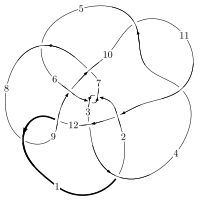
\includegraphics[width=112pt]{../../../GIT/diagram.site/Diagrams/png/1918_12a_1117.png}\\
\ \ \ A knot diagram\footnotemark}&
\allowdisplaybreaks
\textbf{Linearized knot diagam} \\
\cline{2-2}
 &
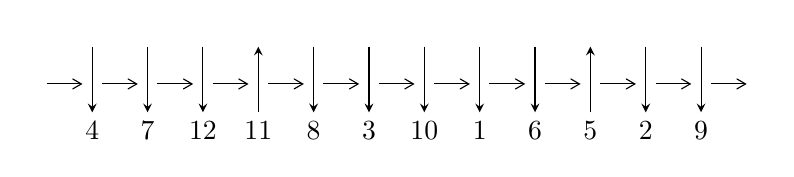
\begin{tikzpicture}[x=20pt, y=17pt]
	% nodes
	\node (C0) at (0, 0) {};
	\node (C1) at (1, 0) {};
	\node (C1U) at (1, +1) {};
	\node (C1D) at (1, -1) {4};

	\node (C2) at (2, 0) {};
	\node (C2U) at (2, +1) {};
	\node (C2D) at (2, -1) {7};

	\node (C3) at (3, 0) {};
	\node (C3U) at (3, +1) {};
	\node (C3D) at (3, -1) {12};

	\node (C4) at (4, 0) {};
	\node (C4U) at (4, +1) {};
	\node (C4D) at (4, -1) {11};

	\node (C5) at (5, 0) {};
	\node (C5U) at (5, +1) {};
	\node (C5D) at (5, -1) {8};

	\node (C6) at (6, 0) {};
	\node (C6U) at (6, +1) {};
	\node (C6D) at (6, -1) {3};

	\node (C7) at (7, 0) {};
	\node (C7U) at (7, +1) {};
	\node (C7D) at (7, -1) {10};

	\node (C8) at (8, 0) {};
	\node (C8U) at (8, +1) {};
	\node (C8D) at (8, -1) {1};

	\node (C9) at (9, 0) {};
	\node (C9U) at (9, +1) {};
	\node (C9D) at (9, -1) {6};

	\node (C10) at (10, 0) {};
	\node (C10U) at (10, +1) {};
	\node (C10D) at (10, -1) {5};

	\node (C11) at (11, 0) {};
	\node (C11U) at (11, +1) {};
	\node (C11D) at (11, -1) {2};

	\node (C12) at (12, 0) {};
	\node (C12U) at (12, +1) {};
	\node (C12D) at (12, -1) {9};
	\node (C13) at (13, 0) {};

	% arrows
	\draw[->,>={angle 60}]
	(C0) edge (C1) (C1) edge (C2) (C2) edge (C3) (C3) edge (C4) (C4) edge (C5) (C5) edge (C6) (C6) edge (C7) (C7) edge (C8) (C8) edge (C9) (C9) edge (C10) (C10) edge (C11) (C11) edge (C12) (C12) edge (C13) ;	\draw[->,>=stealth]
	(C1U) edge (C1D) (C2U) edge (C2D) (C3U) edge (C3D) (C4D) edge (C4U) (C5U) edge (C5D) (C6U) edge (C6D) (C7U) edge (C7D) (C8U) edge (C8D) (C9U) edge (C9D) (C10D) edge (C10U) (C11U) edge (C11D) (C12U) edge (C12D) ;
	\end{tikzpicture} \\
\hhline{~~} \\& 
\textbf{Solving Sequence} \\ \cline{2-2} 
 &
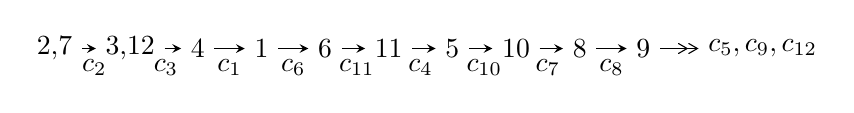
\begin{tikzpicture}[x=23pt, y=7pt]
	% node
	\node (A0) at (-1/8, 0) {2,7};
	\node (A1) at (17/16, 0) {3,12};
	\node (A2) at (17/8, 0) {4};
	\node (A3) at (25/8, 0) {1};
	\node (A4) at (33/8, 0) {6};
	\node (A5) at (41/8, 0) {11};
	\node (A6) at (49/8, 0) {5};
	\node (A7) at (57/8, 0) {10};
	\node (A8) at (65/8, 0) {8};
	\node (A9) at (73/8, 0) {9};
	\node (C1) at (1/2, -1) {$c_{2}$};
	\node (C2) at (13/8, -1) {$c_{3}$};
	\node (C3) at (21/8, -1) {$c_{1}$};
	\node (C4) at (29/8, -1) {$c_{6}$};
	\node (C5) at (37/8, -1) {$c_{11}$};
	\node (C6) at (45/8, -1) {$c_{4}$};
	\node (C7) at (53/8, -1) {$c_{10}$};
	\node (C8) at (61/8, -1) {$c_{7}$};
	\node (C9) at (69/8, -1) {$c_{8}$};
	\node (A10) at (11, 0) {$c_{5},c_{9},c_{12}$};

	% edge
	\draw[->,>=stealth]	
	(A0) edge (A1) (A1) edge (A2) (A2) edge (A3) (A3) edge (A4) (A4) edge (A5) (A5) edge (A6) (A6) edge (A7) (A7) edge (A8) (A8) edge (A9) ;
	\draw[->>,>={angle 60}]	
	(A9) edge (A10);
\end{tikzpicture} \\ 

\end{tabular} \\

\footnotetext{
The image of knot diagram is generated by the software ``\textbf{Draw programme}" developed by Andrew Bartholomew(\url{http://www.layer8.co.uk/maths/draw/index.htm\#Running-draw}), where we modified some parts for our purpose(\url{https://github.com/CATsTAILs/LinksPainter}).
}\phantom \\ \newline 
\centering \textbf{Ideals for irreducible components\footnotemark of $X_{\text{par}}$} 
 
\begin{align*}
I^u_{1}&=\langle 
-1774 u^{14}+1315 u^{13}+\cdots+8515 b+4857,\;421 u^{14}-2705 u^{13}+\cdots+17030 a+2712,\\
\phantom{I^u_{1}}&\phantom{= \langle  }u^{15}- u^{14}+4 u^{13}-3 u^{12}+9 u^{11}-7 u^{10}+8 u^9-4 u^8+2 u^7-2 u^5+11 u^4+7 u^3-2 u^2+4 u-2\rangle \\
I^u_{2}&=\langle 
1.02239\times10^{93} u^{49}-2.36989\times10^{93} u^{48}+\cdots+2.27314\times10^{94} b-4.69141\times10^{94},\\
\phantom{I^u_{2}}&\phantom{= \langle  }-2.13211\times10^{95} u^{49}+7.59053\times10^{95} u^{48}+\cdots+2.84142\times10^{96} a+4.71518\times10^{97},\\
\phantom{I^u_{2}}&\phantom{= \langle  }u^{50}-3 u^{49}+\cdots-957 u+125\rangle \\
I^u_{3}&=\langle 
-1.28305\times10^{63} a u^{37}-2.62014\times10^{63} u^{37}+\cdots+2.14337\times10^{64} a+3.87045\times10^{64},\\
\phantom{I^u_{3}}&\phantom{= \langle  }-7.13697\times10^{65} a u^{37}-1.84375\times10^{66} u^{37}+\cdots-1.34162\times10^{67} a-3.37015\times10^{66},\\
\phantom{I^u_{3}}&\phantom{= \langle  }2 u^{38}-3 u^{37}+\cdots+21 u+17\rangle \\
I^u_{4}&=\langle 
u^7+u^6+3 u^5+2 u^4- u^2 a+3 u^3+u^2+b- a+u+1,\\
\phantom{I^u_{4}}&\phantom{= \langle  }-2 u^7 a-2 u^6 a- u^7-7 u^5 a- u^6-5 u^4 a-2 u^5-8 u^3 a- u^4-3 u^2 a+a^2-3 a u+u^2+u+1,\\
\phantom{I^u_{4}}&\phantom{= \langle  }u^9+u^8+4 u^7+3 u^6+6 u^5+3 u^4+4 u^3+u^2+u-1\rangle \\
I^u_{5}&=\langle 
-2 u^4 a+u^5-4 u^3 a-7 u^2 a- u^3-4 a u-4 u^2+b- a-3 u,\\
\phantom{I^u_{5}}&\phantom{= \langle  }13 u^5 a+13 u^4 a+30 u^5+26 u^3 a+37 u^4+13 u^2 a+86 u^3+13 a^2+13 a u+48 u^2+26 a+65 u+38,\\
\phantom{I^u_{5}}&\phantom{= \langle  }u^6+2 u^5+4 u^4+4 u^3+4 u^2+3 u+1\rangle \\
I^u_{6}&=\langle 
- u^2 a+b-1,\;2 u^5 a- u^5+4 u^3 a-2 u^2 a-2 u^3+a^2+u^2- a,\;u^6+u^5+3 u^4+2 u^3+2 u^2+u+1\rangle \\
I^u_{7}&=\langle 
2 u^5-5 u^4-4 u^2 a+3 u^3-4 a u-6 u^2+8 b-5 u-9,\;-212 u^5 a+110 u^5+\cdots+34 a+133,\\
\phantom{I^u_{7}}&\phantom{= \langle  }2 u^6+u^5+4 u^4+3 u^3+5 u^2+1\rangle \\
I^u_{8}&=\langle 
u^2+b- u+1,\;a+u,\;u^3- u^2+2 u-1\rangle \\
I^u_{9}&=\langle 
u^6-4 u^5+8 u^4-11 u^3+9 u^2+b-5 u+3,\;-3 u^7+10 u^6-17 u^5+18 u^4-7 u^3- u^2+2 a+u-4,\\
\phantom{I^u_{9}}&\phantom{= \langle  }u^8-4 u^7+9 u^6-14 u^5+15 u^4-13 u^3+9 u^2-4 u+2\rangle \\
\\
\end{align*}
\raggedright * 9 irreducible components of $\dim_{\mathbb{C}}=0$, with total 206 representations.\\
\footnotetext{All coefficients of polynomials are rational numbers. But the coefficients are sometimes approximated in decimal forms when there is not enough margin.}
\newpage
\renewcommand{\arraystretch}{1}
\centering \section*{I. $I^u_{1}= \langle -1774 u^{14}+1315 u^{13}+\cdots+8515 b+4857,\;421 u^{14}-2705 u^{13}+\cdots+17030 a+2712,\;u^{15}- u^{14}+\cdots+4 u-2 \rangle$}
\flushleft \textbf{(i) Arc colorings}\\
\begin{tabular}{m{7pt} m{180pt} m{7pt} m{180pt} }
\flushright $a_{2}=$&$\begin{pmatrix}1\\0\end{pmatrix}$ \\
\flushright $a_{7}=$&$\begin{pmatrix}0\\u\end{pmatrix}$ \\
\flushright $a_{3}=$&$\begin{pmatrix}1\\u^2\end{pmatrix}$ \\
\flushright $a_{12}=$&$\begin{pmatrix}-0.0247211 u^{14}+0.158837 u^{13}+\cdots+2.48984 u-0.159248\\0.208338 u^{14}-0.154433 u^{13}+\cdots-0.364416 u-0.570405\end{pmatrix}$ \\
\flushright $a_{4}=$&$\begin{pmatrix}0.135828 u^{14}-0.284588 u^{13}+\cdots-3.28945 u+1.66278\\-0.208338 u^{14}+0.154433 u^{13}+\cdots+0.364416 u+0.570405\end{pmatrix}$ \\
\flushright $a_{1}=$&$\begin{pmatrix}0.0588961 u^{14}+0.355549 u^{13}+\cdots+2.50757 u-0.858133\\0.0723429 u^{14}-0.142689 u^{13}+\cdots-1.52225 u+0.130006\end{pmatrix}$ \\
\flushright $a_{6}=$&$\begin{pmatrix}u\\u^3+u\end{pmatrix}$ \\
\flushright $a_{11}=$&$\begin{pmatrix}0.183617 u^{14}+0.00440399 u^{13}+\cdots+2.12543 u-0.729654\\0.208338 u^{14}-0.154433 u^{13}+\cdots-0.364416 u-0.570405\end{pmatrix}$ \\
\flushright $a_{5}=$&$\begin{pmatrix}-0.251732 u^{14}+0.169407 u^{13}+\cdots+1.00317 u+0.923429\\-0.0823253 u^{14}+0.186729 u^{13}+\cdots+1.93036 u-0.503464\end{pmatrix}$ \\
\flushright $a_{10}=$&$\begin{pmatrix}0.285203 u^{14}-0.493541 u^{13}+\cdots-1.60681 u+1.50523\\-0.188021 u^{14}+0.100998 u^{13}+\cdots+1.46412 u-0.367234\end{pmatrix}$ \\
\flushright $a_{8}=$&$\begin{pmatrix}0.0650029 u^{14}+0.00733999 u^{13}+\cdots+1.10135 u-1.26224\\0.279859 u^{14}-0.352319 u^{13}+\cdots-0.664827 u+0.387669\end{pmatrix}$ \\
\flushright $a_{9}=$&$\begin{pmatrix}-0.349442 u^{14}+0.433059 u^{13}+\cdots+2.19507 u-1.38004\\0.350206 u^{14}-0.486201 u^{13}+\cdots-0.505461 u+0.242983\end{pmatrix}$\\&\end{tabular}
\flushleft \textbf{(ii) Obstruction class $= -1$}\\~\\
\flushleft \textbf{(iii) Cusp Shapes $= -\frac{1436398}{1439035} u^{14}+\frac{520186}{287807} u^{13}+\cdots+\frac{10729646}{1439035} u-\frac{16780726}{1439035}$}\\~\\
\newpage\renewcommand{\arraystretch}{1}
\flushleft \textbf{(iv) u-Polynomials at the component}\newline \\
\begin{tabular}{m{50pt}|m{274pt}}
Crossings & \hspace{64pt}u-Polynomials at each crossing \\
\hline $$\begin{aligned}c_{1},c_{5},c_{7}\\c_{11}\end{aligned}$$&$\begin{aligned}
&u^{15}+3 u^{12}+\cdots+40 u+13
\end{aligned}$\\
\hline $$\begin{aligned}c_{2},c_{6},c_{8}\\c_{12}\end{aligned}$$&$\begin{aligned}
&u^{15}+u^{14}+\cdots+4 u+2
\end{aligned}$\\
\hline $$\begin{aligned}c_{3},c_{9}\end{aligned}$$&$\begin{aligned}
&13(13 u^{15}+127 u^{14}+\cdots+224 u+64)
\end{aligned}$\\
\hline $$\begin{aligned}c_{4},c_{10}\end{aligned}$$&$\begin{aligned}
&13(13 u^{15}+127 u^{14}+\cdots+672 u+64)
\end{aligned}$\\
\hline
\end{tabular}\\~\\
\newpage\renewcommand{\arraystretch}{1}
\flushleft \textbf{(v) Riley Polynomials at the component}\newline \\
\begin{tabular}{m{50pt}|m{274pt}}
Crossings & \hspace{64pt}Riley Polynomials at each crossing \\
\hline $$\begin{aligned}c_{1},c_{5},c_{7}\\c_{11}\end{aligned}$$&$\begin{aligned}
&y^{15}+18 y^{13}+\cdots+768 y-169
\end{aligned}$\\
\hline $$\begin{aligned}c_{2},c_{6},c_{8}\\c_{12}\end{aligned}$$&$\begin{aligned}
&y^{15}+7 y^{14}+\cdots+8 y-4
\end{aligned}$\\
\hline $$\begin{aligned}c_{3},c_{9}\end{aligned}$$&$\begin{aligned}
&169(169 y^{15}-425 y^{14}+\cdots+13312 y-4096)
\end{aligned}$\\
\hline $$\begin{aligned}c_{4},c_{10}\end{aligned}$$&$\begin{aligned}
&169(169 y^{15}+1265 y^{14}+\cdots+35840 y-4096)
\end{aligned}$\\
\hline
\end{tabular}\\~\\
\newpage\flushleft \textbf{(vi) Complex Volumes and Cusp Shapes}
$$\begin{array}{c|c|c}  
\text{Solutions to }I^u_{1}& \I (\text{vol} + \sqrt{-1}CS) & \text{Cusp shape}\\
 \hline 
\begin{aligned}
u &= \phantom{-}1.038030 + 0.415186 I \\
a &= -0.107387 + 0.237703 I \\
b &= -1.18691 + 0.94003 I\end{aligned}
 & -6.76596 + 8.23973 I & -12.44890 - 5.51988 I \\ \hline\begin{aligned}
u &= \phantom{-}1.038030 - 0.415186 I \\
a &= -0.107387 - 0.237703 I \\
b &= -1.18691 - 0.94003 I\end{aligned}
 & -6.76596 - 8.23973 I & -12.44890 + 5.51988 I \\ \hline\begin{aligned}
u &= -0.818246 + 0.256414 I \\
a &= \phantom{-}0.119221 + 0.079347 I \\
b &= -0.746763 - 0.703405 I\end{aligned}
 & -1.27634 - 4.00007 I & -9.95322 + 5.67504 I \\ \hline\begin{aligned}
u &= -0.818246 - 0.256414 I \\
a &= \phantom{-}0.119221 - 0.079347 I \\
b &= -0.746763 + 0.703405 I\end{aligned}
 & -1.27634 + 4.00007 I & -9.95322 - 5.67504 I \\ \hline\begin{aligned}
u &= -0.582500 + 1.172270 I \\
a &= -0.726702 - 0.702424 I \\
b &= \phantom{-}0.232232 + 1.055820 I\end{aligned}
 & \phantom{-}5.94870 + 3.89270 I & \phantom{-}1.63186 - 3.82155 I \\ \hline\begin{aligned}
u &= -0.582500 - 1.172270 I \\
a &= -0.726702 + 0.702424 I \\
b &= \phantom{-}0.232232 - 1.055820 I\end{aligned}
 & \phantom{-}5.94870 - 3.89270 I & \phantom{-}1.63186 + 3.82155 I \\ \hline\begin{aligned}
u &= -0.630803 + 1.198390 I \\
a &= \phantom{-}0.37453 + 1.69980 I \\
b &= \phantom{-}0.879361 - 0.931227 I\end{aligned}
 & \phantom{-}4.1064 + 14.7431 I & -5.12518 - 11.18062 I \\ \hline\begin{aligned}
u &= -0.630803 - 1.198390 I \\
a &= \phantom{-}0.37453 - 1.69980 I \\
b &= \phantom{-}0.879361 + 0.931227 I\end{aligned}
 & \phantom{-}4.1064 - 14.7431 I & -5.12518 + 11.18062 I \\ \hline\begin{aligned}
u &= \phantom{-}0.053320 + 0.620675 I \\
a &= -1.04030 + 1.99312 I \\
b &= -0.984982 - 0.608770 I\end{aligned}
 & -3.34242 - 5.61099 I & -7.68675 + 5.73270 I \\ \hline\begin{aligned}
u &= \phantom{-}0.053320 - 0.620675 I \\
a &= -1.04030 - 1.99312 I \\
b &= -0.984982 + 0.608770 I\end{aligned}
 & -3.34242 + 5.61099 I & -7.68675 - 5.73270 I\\
 \hline 
 \end{array}$$\newpage$$\begin{array}{c|c|c}  
\text{Solutions to }I^u_{1}& \I (\text{vol} + \sqrt{-1}CS) & \text{Cusp shape}\\
 \hline 
\begin{aligned}
u &= \phantom{-}0.501612 + 1.316920 I \\
a &= -0.603038 + 0.494954 I \\
b &= \phantom{-}0.696809 - 1.108770 I\end{aligned}
 & \phantom{-}3.12015 - 0.43357 I & -3.52219 - 1.71416 I \\ \hline\begin{aligned}
u &= \phantom{-}0.501612 - 1.316920 I \\
a &= -0.603038 - 0.494954 I \\
b &= \phantom{-}0.696809 + 1.108770 I\end{aligned}
 & \phantom{-}3.12015 + 0.43357 I & -3.52219 + 1.71416 I \\ \hline\begin{aligned}
u &= \phantom{-}0.73808 + 1.30226 I \\
a &= \phantom{-}0.33381 - 1.50205 I \\
b &= \phantom{-}1.32262 + 1.06232 I\end{aligned}
 & -1.3169 - 21.4322 I & -8.08580 + 10.72948 I \\ \hline\begin{aligned}
u &= \phantom{-}0.73808 - 1.30226 I \\
a &= \phantom{-}0.33381 + 1.50205 I \\
b &= \phantom{-}1.32262 - 1.06232 I\end{aligned}
 & -1.3169 + 21.4322 I & -8.08580 - 10.72948 I \\ \hline\begin{aligned}
u &= \phantom{-}0.401015\phantom{ +0.000000I} \\
a &= \phantom{-}1.22281\phantom{ +0.000000I} \\
b &= -0.424742\phantom{ +0.000000I}\end{aligned}
 & -0.947362\phantom{ +0.000000I} & -10.6110\phantom{ +0.000000I}\\
 \hline 
 \end{array}$$\newpage\newpage\renewcommand{\arraystretch}{1}
\centering \section*{II. $I^u_{2}= \langle 1.02\times10^{93} u^{49}-2.37\times10^{93} u^{48}+\cdots+2.27\times10^{94} b-4.69\times10^{94},\;-2.13\times10^{95} u^{49}+7.59\times10^{95} u^{48}+\cdots+2.84\times10^{96} a+4.72\times10^{97},\;u^{50}-3 u^{49}+\cdots-957 u+125 \rangle$}
\flushleft \textbf{(i) Arc colorings}\\
\begin{tabular}{m{7pt} m{180pt} m{7pt} m{180pt} }
\flushright $a_{2}=$&$\begin{pmatrix}1\\0\end{pmatrix}$ \\
\flushright $a_{7}=$&$\begin{pmatrix}0\\u\end{pmatrix}$ \\
\flushright $a_{3}=$&$\begin{pmatrix}1\\u^2\end{pmatrix}$ \\
\flushright $a_{12}=$&$\begin{pmatrix}0.0750367 u^{49}-0.267139 u^{48}+\cdots+114.350 u-16.5944\\-0.0449772 u^{49}+0.104256 u^{48}+\cdots-10.0854 u+2.06385\end{pmatrix}$ \\
\flushright $a_{4}=$&$\begin{pmatrix}-0.105135 u^{49}+0.507258 u^{48}+\cdots-294.562 u+45.6110\\-0.00353631 u^{49}+0.0153181 u^{48}+\cdots-2.87629 u+0.356571\end{pmatrix}$ \\
\flushright $a_{1}=$&$\begin{pmatrix}-0.0323039 u^{49}+0.0449478 u^{48}+\cdots+25.2923 u-1.57484\\0.00276577 u^{49}-0.00285242 u^{48}+\cdots+1.62853 u-0.570441\end{pmatrix}$ \\
\flushright $a_{6}=$&$\begin{pmatrix}u\\u^3+u\end{pmatrix}$ \\
\flushright $a_{11}=$&$\begin{pmatrix}0.0300595 u^{49}-0.162882 u^{48}+\cdots+104.264 u-14.5306\\-0.0449772 u^{49}+0.104256 u^{48}+\cdots-10.0854 u+2.06385\end{pmatrix}$ \\
\flushright $a_{5}=$&$\begin{pmatrix}-0.0372083 u^{49}+0.116277 u^{48}+\cdots-56.4918 u+7.97128\\0.00465181 u^{49}+0.0233411 u^{48}+\cdots-27.6371 u+4.65104\end{pmatrix}$ \\
\flushright $a_{10}=$&$\begin{pmatrix}0.0165108 u^{49}-0.00455519 u^{48}+\cdots+10.6297 u-5.71548\\0.0727039 u^{49}-0.145011 u^{48}+\cdots-14.2364 u+3.75744\end{pmatrix}$ \\
\flushright $a_{8}=$&$\begin{pmatrix}-0.0355511 u^{49}+0.0403247 u^{48}+\cdots+33.8998 u-5.13149\\-0.0608665 u^{49}+0.155509 u^{48}+\cdots-32.2651 u+3.01319\end{pmatrix}$ \\
\flushright $a_{9}=$&$\begin{pmatrix}-0.0112339 u^{49}+0.0339683 u^{48}+\cdots-48.1295 u+11.0302\\-0.0250331 u^{49}+0.0529219 u^{48}+\cdots+19.3755 u-4.09822\end{pmatrix}$\\&\end{tabular}
\flushleft \textbf{(ii) Obstruction class $= -1$}\\~\\
\flushleft \textbf{(iii) Cusp Shapes $= 3.05039 u^{49}-8.14878 u^{48}+\cdots+2125.58 u-268.153$}\\~\\
\newpage\renewcommand{\arraystretch}{1}
\flushleft \textbf{(iv) u-Polynomials at the component}\newline \\
\begin{tabular}{m{50pt}|m{274pt}}
Crossings & \hspace{64pt}u-Polynomials at each crossing \\
\hline $$\begin{aligned}c_{1},c_{5},c_{7}\\c_{11}\end{aligned}$$&$\begin{aligned}
&u^{50}- u^{49}+\cdots+20 u+4
\end{aligned}$\\
\hline $$\begin{aligned}c_{2},c_{6},c_{8}\\c_{12}\end{aligned}$$&$\begin{aligned}
&u^{50}+3 u^{49}+\cdots+957 u+125
\end{aligned}$\\
\hline $$\begin{aligned}c_{3},c_{9}\end{aligned}$$&$\begin{aligned}
&(u^{25}-7 u^{23}+\cdots+u+1)^{2}
\end{aligned}$\\
\hline $$\begin{aligned}c_{4},c_{10}\end{aligned}$$&$\begin{aligned}
&(u^{25}+u^{24}+\cdots-8 u+8)^{2}
\end{aligned}$\\
\hline
\end{tabular}\\~\\
\newpage\renewcommand{\arraystretch}{1}
\flushleft \textbf{(v) Riley Polynomials at the component}\newline \\
\begin{tabular}{m{50pt}|m{274pt}}
Crossings & \hspace{64pt}Riley Polynomials at each crossing \\
\hline $$\begin{aligned}c_{1},c_{5},c_{7}\\c_{11}\end{aligned}$$&$\begin{aligned}
&y^{50}-11 y^{49}+\cdots+448 y+16
\end{aligned}$\\
\hline $$\begin{aligned}c_{2},c_{6},c_{8}\\c_{12}\end{aligned}$$&$\begin{aligned}
&y^{50}+19 y^{49}+\cdots-73349 y+15625
\end{aligned}$\\
\hline $$\begin{aligned}c_{3},c_{9}\end{aligned}$$&$\begin{aligned}
&(y^{25}-14 y^{24}+\cdots-13 y-1)^{2}
\end{aligned}$\\
\hline $$\begin{aligned}c_{4},c_{10}\end{aligned}$$&$\begin{aligned}
&(y^{25}-7 y^{24}+\cdots-1312 y-64)^{2}
\end{aligned}$\\
\hline
\end{tabular}\\~\\
\newpage\flushleft \textbf{(vi) Complex Volumes and Cusp Shapes}
$$\begin{array}{c|c|c}  
\text{Solutions to }I^u_{2}& \I (\text{vol} + \sqrt{-1}CS) & \text{Cusp shape}\\
 \hline 
\begin{aligned}
u &= -0.962281 + 0.315271 I \\
a &= \phantom{-}0.039372 - 0.397643 I \\
b &= \phantom{-}0.810487 + 0.733899 I\end{aligned}
 & \phantom{-}1.42815 - 8.97153 I & -6.72568 + 8.57221 I \\ \hline\begin{aligned}
u &= -0.962281 - 0.315271 I \\
a &= \phantom{-}0.039372 + 0.397643 I \\
b &= \phantom{-}0.810487 - 0.733899 I\end{aligned}
 & \phantom{-}1.42815 + 8.97153 I & -6.72568 - 8.57221 I \\ \hline\begin{aligned}
u &= \phantom{-}0.493412 + 0.847894 I \\
a &= -2.46208 - 4.61887 I \\
b &= -0.114573 + 0.136054 I\end{aligned}
 & \phantom{-}0.0113486\phantom{ +0.000000I} & -289.859 + 0. I\phantom{ +0.000000I} \\ \hline\begin{aligned}
u &= \phantom{-}0.493412 - 0.847894 I \\
a &= -2.46208 + 4.61887 I \\
b &= -0.114573 - 0.136054 I\end{aligned}
 & \phantom{-}0.0113486\phantom{ +0.000000I} & -289.859 + 0. I\phantom{ +0.000000I} \\ \hline\begin{aligned}
u &= \phantom{-}0.946964 + 0.384547 I \\
a &= \phantom{-}0.712275 - 0.392895 I \\
b &= \phantom{-}0.985125 + 0.661648 I\end{aligned}
 & -0.15061 - 5.36191 I & -7.12834 + 6.24088 I \\ \hline\begin{aligned}
u &= \phantom{-}0.946964 - 0.384547 I \\
a &= \phantom{-}0.712275 + 0.392895 I \\
b &= \phantom{-}0.985125 - 0.661648 I\end{aligned}
 & -0.15061 + 5.36191 I & -7.12834 - 6.24088 I \\ \hline\begin{aligned}
u &= \phantom{-}0.601348 + 0.838260 I \\
a &= \phantom{-}0.208165 + 1.190200 I \\
b &= -1.55792 + 0.01038 I\end{aligned}
 & -5.63520 - 2.36394 I & -15.9843 + 4.4825 I \\ \hline\begin{aligned}
u &= \phantom{-}0.601348 - 0.838260 I \\
a &= \phantom{-}0.208165 - 1.190200 I \\
b &= -1.55792 - 0.01038 I\end{aligned}
 & -5.63520 + 2.36394 I & -15.9843 - 4.4825 I \\ \hline\begin{aligned}
u &= \phantom{-}0.313305 + 0.881758 I \\
a &= \phantom{-}0.70859 + 2.12070 I \\
b &= -1.95477 - 0.19516 I\end{aligned}
 & -3.73498 - 1.36050 I & -1.10822 - 1.97856 I \\ \hline\begin{aligned}
u &= \phantom{-}0.313305 - 0.881758 I \\
a &= \phantom{-}0.70859 - 2.12070 I \\
b &= -1.95477 + 0.19516 I\end{aligned}
 & -3.73498 + 1.36050 I & -1.10822 + 1.97856 I\\
 \hline 
 \end{array}$$\newpage$$\begin{array}{c|c|c}  
\text{Solutions to }I^u_{2}& \I (\text{vol} + \sqrt{-1}CS) & \text{Cusp shape}\\
 \hline 
\begin{aligned}
u &= \phantom{-}0.249090 + 1.047960 I \\
a &= -0.63091 + 1.48019 I \\
b &= \phantom{-}0.739655 - 0.926973 I\end{aligned}
 & \phantom{-}1.45153 - 5.02987 I & -7.30473 + 4.45843 I \\ \hline\begin{aligned}
u &= \phantom{-}0.249090 - 1.047960 I \\
a &= -0.63091 - 1.48019 I \\
b &= \phantom{-}0.739655 + 0.926973 I\end{aligned}
 & \phantom{-}1.45153 + 5.02987 I & -7.30473 - 4.45843 I \\ \hline\begin{aligned}
u &= -0.242281 + 1.086980 I \\
a &= \phantom{-}0.759622 + 0.980906 I \\
b &= -0.117932 - 0.819072 I\end{aligned}
 & \phantom{-}3.28228 - 1.03639 I & -2.01858 + 2.13545 I \\ \hline\begin{aligned}
u &= -0.242281 - 1.086980 I \\
a &= \phantom{-}0.759622 - 0.980906 I \\
b &= -0.117932 + 0.819072 I\end{aligned}
 & \phantom{-}3.28228 + 1.03639 I & -2.01858 - 2.13545 I \\ \hline\begin{aligned}
u &= -0.170002 + 0.849577 I \\
a &= \phantom{-}0.47091 - 1.81641 I \\
b &= -1.269920 + 0.483777 I\end{aligned}
 & -0.954576 + 1.006090 I & -21.6904 - 0.7850 I \\ \hline\begin{aligned}
u &= -0.170002 - 0.849577 I \\
a &= \phantom{-}0.47091 + 1.81641 I \\
b &= -1.269920 - 0.483777 I\end{aligned}
 & -0.954576 - 1.006090 I & -21.6904 + 0.7850 I \\ \hline\begin{aligned}
u &= \phantom{-}0.706085 + 0.894642 I \\
a &= \phantom{-}0.713820 - 0.553959 I \\
b &= \phantom{-}0.571998 + 0.140311 I\end{aligned}
 & -1.32757 - 2.72807 I & -8.00000 + 0. I\phantom{ +0.000000I} \\ \hline\begin{aligned}
u &= \phantom{-}0.706085 - 0.894642 I \\
a &= \phantom{-}0.713820 + 0.553959 I \\
b &= \phantom{-}0.571998 - 0.140311 I\end{aligned}
 & -1.32757 + 2.72807 I & -8.00000 + 0. I\phantom{ +0.000000I} \\ \hline\begin{aligned}
u &= -1.180310 + 0.078417 I \\
a &= \phantom{-}0.213834 - 0.613152 I \\
b &= -0.103922 - 0.683562 I\end{aligned}
 & -5.63520 - 2.36394 I & -15.9843 + 4.4825 I \\ \hline\begin{aligned}
u &= -1.180310 - 0.078417 I \\
a &= \phantom{-}0.213834 + 0.613152 I \\
b &= -0.103922 + 0.683562 I\end{aligned}
 & -5.63520 + 2.36394 I & -15.9843 - 4.4825 I\\
 \hline 
 \end{array}$$\newpage$$\begin{array}{c|c|c}  
\text{Solutions to }I^u_{2}& \I (\text{vol} + \sqrt{-1}CS) & \text{Cusp shape}\\
 \hline 
\begin{aligned}
u &= \phantom{-}0.074692 + 1.200860 I \\
a &= \phantom{-}0.686373 - 1.101630 I \\
b &= -0.622763 + 1.268480 I\end{aligned}
 & -0.15061 + 5.36191 I & -8.00000 + 0. I\phantom{ +0.000000I} \\ \hline\begin{aligned}
u &= \phantom{-}0.074692 - 1.200860 I \\
a &= \phantom{-}0.686373 + 1.101630 I \\
b &= -0.622763 - 1.268480 I\end{aligned}
 & -0.15061 - 5.36191 I & -8.00000 + 0. I\phantom{ +0.000000I} \\ \hline\begin{aligned}
u &= \phantom{-}0.390389 + 1.160270 I \\
a &= -0.14604 - 1.82543 I \\
b &= \phantom{-}1.58187 + 0.79235 I\end{aligned}
 & \phantom{-}4.19376 - 8.71277 I & \phantom{-0.000000 } 0 \\ \hline\begin{aligned}
u &= \phantom{-}0.390389 - 1.160270 I \\
a &= -0.14604 + 1.82543 I \\
b &= \phantom{-}1.58187 - 0.79235 I\end{aligned}
 & \phantom{-}4.19376 + 8.71277 I & \phantom{-0.000000 } 0 \\ \hline\begin{aligned}
u &= -0.743476 + 0.164819 I \\
a &= \phantom{-}0.655758 + 0.108650 I \\
b &= \phantom{-}0.589628 - 0.786025 I\end{aligned}
 & \phantom{-}3.28228 + 1.03639 I & -2.01858 - 2.13545 I \\ \hline\begin{aligned}
u &= -0.743476 - 0.164819 I \\
a &= \phantom{-}0.655758 - 0.108650 I \\
b &= \phantom{-}0.589628 + 0.786025 I\end{aligned}
 & \phantom{-}3.28228 - 1.03639 I & -2.01858 + 2.13545 I \\ \hline\begin{aligned}
u &= \phantom{-}1.223420 + 0.291121 I \\
a &= \phantom{-}0.061981 - 0.257278 I \\
b &= -0.148168 + 0.319622 I\end{aligned}
 & -0.954576 - 1.006090 I & \phantom{-0.000000 } 0 \\ \hline\begin{aligned}
u &= \phantom{-}1.223420 - 0.291121 I \\
a &= \phantom{-}0.061981 + 0.257278 I \\
b &= -0.148168 - 0.319622 I\end{aligned}
 & -0.954576 + 1.006090 I & \phantom{-0.000000 } 0 \\ \hline\begin{aligned}
u &= -0.535150 + 1.155570 I \\
a &= -0.24384 - 1.72241 I \\
b &= -0.855287 + 1.021820 I\end{aligned}
 & \phantom{-}1.42815 + 8.97153 I & \phantom{-0.000000 } 0 \\ \hline\begin{aligned}
u &= -0.535150 - 1.155570 I \\
a &= -0.24384 + 1.72241 I \\
b &= -0.855287 - 1.021820 I\end{aligned}
 & \phantom{-}1.42815 - 8.97153 I & \phantom{-0.000000 } 0\\
 \hline 
 \end{array}$$\newpage$$\begin{array}{c|c|c}  
\text{Solutions to }I^u_{2}& \I (\text{vol} + \sqrt{-1}CS) & \text{Cusp shape}\\
 \hline 
\begin{aligned}
u &= -0.372106 + 1.237480 I \\
a &= \phantom{-}0.11902 + 1.61329 I \\
b &= \phantom{-}1.05126 - 1.02792 I\end{aligned}
 & \phantom{-}7.40741 + 4.94924 I & \phantom{-0.000000 } 0 \\ \hline\begin{aligned}
u &= -0.372106 - 1.237480 I \\
a &= \phantom{-}0.11902 - 1.61329 I \\
b &= \phantom{-}1.05126 + 1.02792 I\end{aligned}
 & \phantom{-}7.40741 - 4.94924 I & \phantom{-0.000000 } 0 \\ \hline\begin{aligned}
u &= \phantom{-}1.291650 + 0.403695 I \\
a &= \phantom{-}0.1203380 + 0.0039571 I \\
b &= \phantom{-}1.09552 - 0.98588 I\end{aligned}
 & -4.2488 + 14.3474 I & \phantom{-0.000000 } 0 \\ \hline\begin{aligned}
u &= \phantom{-}1.291650 - 0.403695 I \\
a &= \phantom{-}0.1203380 - 0.0039571 I \\
b &= \phantom{-}1.09552 + 0.98588 I\end{aligned}
 & -4.2488 - 14.3474 I & \phantom{-0.000000 } 0 \\ \hline\begin{aligned}
u &= \phantom{-}0.755348 + 1.140700 I \\
a &= -0.389887 + 0.934449 I \\
b &= -0.466731 - 0.418496 I\end{aligned}
 & \phantom{-}1.45153 - 5.02987 I & \phantom{-0.000000 } 0 \\ \hline\begin{aligned}
u &= \phantom{-}0.755348 - 1.140700 I \\
a &= -0.389887 - 0.934449 I \\
b &= -0.466731 + 0.418496 I\end{aligned}
 & \phantom{-}1.45153 + 5.02987 I & \phantom{-0.000000 } 0 \\ \hline\begin{aligned}
u &= \phantom{-}0.659409 + 1.203940 I \\
a &= -0.32021 + 1.67118 I \\
b &= -1.41005 - 1.08673 I\end{aligned}
 & -4.2488 - 14.3474 I & \phantom{-0.000000 } 0 \\ \hline\begin{aligned}
u &= \phantom{-}0.659409 - 1.203940 I \\
a &= -0.32021 - 1.67118 I \\
b &= -1.41005 + 1.08673 I\end{aligned}
 & -4.2488 + 14.3474 I & \phantom{-0.000000 } 0 \\ \hline\begin{aligned}
u &= \phantom{-}0.072477 + 0.606484 I \\
a &= -1.03463 - 2.22816 I \\
b &= \phantom{-}1.400570 - 0.171399 I\end{aligned}
 & \phantom{-}1.57283 + 6.25459 I & -7.09425 - 6.20570 I \\ \hline\begin{aligned}
u &= \phantom{-}0.072477 - 0.606484 I \\
a &= -1.03463 + 2.22816 I \\
b &= \phantom{-}1.400570 + 0.171399 I\end{aligned}
 & \phantom{-}1.57283 - 6.25459 I & -7.09425 + 6.20570 I\\
 \hline 
 \end{array}$$\newpage$$\begin{array}{c|c|c}  
\text{Solutions to }I^u_{2}& \I (\text{vol} + \sqrt{-1}CS) & \text{Cusp shape}\\
 \hline 
\begin{aligned}
u &= -0.14698 + 1.41040 I \\
a &= -0.494719 - 0.953376 I \\
b &= \phantom{-}0.309442 + 0.752193 I\end{aligned}
 & \phantom{-}7.40741 - 4.94924 I & \phantom{-0.000000 } 0 \\ \hline\begin{aligned}
u &= -0.14698 - 1.41040 I \\
a &= -0.494719 + 0.953376 I \\
b &= \phantom{-}0.309442 - 0.752193 I\end{aligned}
 & \phantom{-}7.40741 + 4.94924 I & \phantom{-0.000000 } 0 \\ \hline\begin{aligned}
u &= -0.49243 + 1.50322 I \\
a &= -0.041335 - 1.053700 I \\
b &= -0.64704 + 1.29841 I\end{aligned}
 & \phantom{-}1.57283 + 6.25459 I & \phantom{-0.000000 } 0 \\ \hline\begin{aligned}
u &= -0.49243 - 1.50322 I \\
a &= -0.041335 + 1.053700 I \\
b &= -0.64704 - 1.29841 I\end{aligned}
 & \phantom{-}1.57283 - 6.25459 I & \phantom{-0.000000 } 0 \\ \hline\begin{aligned}
u &= \phantom{-}0.334545 + 0.056281 I \\
a &= \phantom{-}0.80170 + 1.41679 I \\
b &= \phantom{-}0.121420 - 0.744450 I\end{aligned}
 & -1.32757 - 2.72807 I & -5.71643 + 1.76366 I \\ \hline\begin{aligned}
u &= \phantom{-}0.334545 - 0.056281 I \\
a &= \phantom{-}0.80170 - 1.41679 I \\
b &= \phantom{-}0.121420 + 0.744450 I\end{aligned}
 & -1.32757 + 2.72807 I & -5.71643 - 1.76366 I \\ \hline\begin{aligned}
u &= -1.69246 + 0.17139 I \\
a &= \phantom{-}0.0901819 - 0.0534982 I \\
b &= -0.077041 - 1.057990 I\end{aligned}
 & -3.73498 + 1.36050 I & \phantom{-0.000000 } 0 \\ \hline\begin{aligned}
u &= -1.69246 - 0.17139 I \\
a &= \phantom{-}0.0901819 + 0.0534982 I \\
b &= -0.077041 + 1.057990 I\end{aligned}
 & -3.73498 - 1.36050 I & \phantom{-0.000000 } 0 \\ \hline\begin{aligned}
u &= -0.07465 + 1.74368 I \\
a &= -0.202288 + 0.850448 I \\
b &= \phantom{-}0.589151 - 1.273730 I\end{aligned}
 & \phantom{-}4.19376 + 8.71277 I & \phantom{-0.000000 } 0 \\ \hline\begin{aligned}
u &= -0.07465 - 1.74368 I \\
a &= -0.202288 - 0.850448 I \\
b &= \phantom{-}0.589151 + 1.273730 I\end{aligned}
 & \phantom{-}4.19376 - 8.71277 I & \phantom{-0.000000 } 0\\
 \hline 
 \end{array}$$\newpage\newpage\renewcommand{\arraystretch}{1}
\centering \section*{III. $I^u_{3}= \langle -1.28\times10^{63} a u^{37}-2.62\times10^{63} u^{37}+\cdots+2.14\times10^{64} a+3.87\times10^{64},\;-7.14\times10^{65} a u^{37}-1.84\times10^{66} u^{37}+\cdots-1.34\times10^{67} a-3.37\times10^{66},\;2 u^{38}-3 u^{37}+\cdots+21 u+17 \rangle$}
\flushleft \textbf{(i) Arc colorings}\\
\begin{tabular}{m{7pt} m{180pt} m{7pt} m{180pt} }
\flushright $a_{2}=$&$\begin{pmatrix}1\\0\end{pmatrix}$ \\
\flushright $a_{7}=$&$\begin{pmatrix}0\\u\end{pmatrix}$ \\
\flushright $a_{3}=$&$\begin{pmatrix}1\\u^2\end{pmatrix}$ \\
\flushright $a_{12}=$&$\begin{pmatrix}a\\0.106339 a u^{37}+0.217158 u^{37}+\cdots-1.77643 a-3.20783\end{pmatrix}$ \\
\flushright $a_{4}=$&$\begin{pmatrix}-0.0534232 a u^{37}-0.392917 u^{37}+\cdots+4.95562 a+7.59732\\-0.0962820 a u^{37}-0.180215 u^{37}+\cdots+0.906877 a+0.780461\end{pmatrix}$ \\
\flushright $a_{1}=$&$\begin{pmatrix}0.216255 a u^{37}+1.23930 u^{37}+\cdots-3.28167 a-6.64201\\0.129769 a u^{37}+0.552372 u^{37}+\cdots-0.715136 a+1.66440\end{pmatrix}$ \\
\flushright $a_{6}=$&$\begin{pmatrix}u\\u^3+u\end{pmatrix}$ \\
\flushright $a_{11}=$&$\begin{pmatrix}0.106339 a u^{37}+0.217158 u^{37}+\cdots-0.776427 a-3.20783\\0.106339 a u^{37}+0.217158 u^{37}+\cdots-1.77643 a-3.20783\end{pmatrix}$ \\
\flushright $a_{5}=$&$\begin{pmatrix}-0.182671 a u^{37}-0.726160 u^{37}+\cdots+2.16849 a+1.45704\\-0.201850 a u^{37}-0.513458 u^{37}+\cdots-1.55270 a-5.35982\end{pmatrix}$ \\
\flushright $a_{10}=$&$\begin{pmatrix}0.208991 a u^{37}+0.272662 u^{37}+\cdots+1.92898 a+7.20364\\-0.152476 a u^{37}-0.486462 u^{37}+\cdots-0.903884 a-0.470790\end{pmatrix}$ \\
\flushright $a_{8}=$&$\begin{pmatrix}0.0694187 a u^{37}+0.849176 u^{37}+\cdots+1.65114 a+15.0369\\0.149109 a u^{37}+0.212456 u^{37}+\cdots+2.61168 a+8.33710\end{pmatrix}$ \\
\flushright $a_{9}=$&$\begin{pmatrix}-0.361467 a u^{37}-0.529227 u^{37}+\cdots-2.83287 a-7.65774\\0.0845476 a u^{37}+0.366409 u^{37}+\cdots+0.172876 a-0.233667\end{pmatrix}$\\&\end{tabular}
\flushleft \textbf{(ii) Obstruction class $= -1$}\\~\\
\flushleft \textbf{(iii) Cusp Shapes $= -0.432764 u^{37}+1.23037 u^{36}+\cdots+6.30892 u-4.51753$}\\~\\
\newpage\renewcommand{\arraystretch}{1}
\flushleft \textbf{(iv) u-Polynomials at the component}\newline \\
\begin{tabular}{m{50pt}|m{274pt}}
Crossings & \hspace{64pt}u-Polynomials at each crossing \\
\hline $$\begin{aligned}c_{1},c_{5},c_{7}\\c_{11}\end{aligned}$$&$\begin{aligned}
&8(8 u^{76}-90 u^{75}+\cdots-4995 u+404)
\end{aligned}$\\
\hline $$\begin{aligned}c_{2},c_{6},c_{8}\\c_{12}\end{aligned}$$&$\begin{aligned}
&4(2 u^{38}+3 u^{37}+\cdots-21 u+17)^{2}
\end{aligned}$\\
\hline $$\begin{aligned}c_{3},c_{9}\end{aligned}$$&$\begin{aligned}
&4(2 u^{38}-9 u^{37}+\cdots-13 u+4)^{2}
\end{aligned}$\\
\hline $$\begin{aligned}c_{4},c_{10}\end{aligned}$$&$\begin{aligned}
&(u^{19}-2 u^{18}+\cdots-2 u-1)^{4}
\end{aligned}$\\
\hline
\end{tabular}\\~\\
\newpage\renewcommand{\arraystretch}{1}
\flushleft \textbf{(v) Riley Polynomials at the component}\newline \\
\begin{tabular}{m{50pt}|m{274pt}}
Crossings & \hspace{64pt}Riley Polynomials at each crossing \\
\hline $$\begin{aligned}c_{1},c_{5},c_{7}\\c_{11}\end{aligned}$$&$\begin{aligned}
&64(64 y^{76}-980 y^{75}+\cdots+3.63279\times10^{7} y+163216)
\end{aligned}$\\
\hline $$\begin{aligned}c_{2},c_{6},c_{8}\\c_{12}\end{aligned}$$&$\begin{aligned}
&16(4 y^{38}+79 y^{37}+\cdots+2959 y+289)^{2}
\end{aligned}$\\
\hline $$\begin{aligned}c_{3},c_{9}\end{aligned}$$&$\begin{aligned}
&16(4 y^{38}-41 y^{37}+\cdots+455 y+16)^{2}
\end{aligned}$\\
\hline $$\begin{aligned}c_{4},c_{10}\end{aligned}$$&$\begin{aligned}
&(y^{19}+14 y^{18}+\cdots-12 y-1)^{4}
\end{aligned}$\\
\hline
\end{tabular}\\~\\
\newpage\flushleft \textbf{(vi) Complex Volumes and Cusp Shapes}
$$\begin{array}{c|c|c}  
\text{Solutions to }I^u_{3}& \I (\text{vol} + \sqrt{-1}CS) & \text{Cusp shape}\\
 \hline 
\begin{aligned}
u &= \phantom{-}0.933781 + 0.188280 I \\
a &= \phantom{-}0.105927 - 0.244777 I \\
b &= \phantom{-}0.996480 + 0.475628 I\end{aligned}
 & -3.98037 - 6.82755 I & -13.3540 + 7.7872 I \\ \hline\begin{aligned}
u &= \phantom{-}0.933781 + 0.188280 I \\
a &= \phantom{-}1.66297 - 0.60548 I \\
b &= \phantom{-}1.020730 - 0.881690 I\end{aligned}
 & -3.98037 - 6.82755 I & -13.3540 + 7.7872 I \\ \hline\begin{aligned}
u &= \phantom{-}0.933781 - 0.188280 I \\
a &= \phantom{-}0.105927 + 0.244777 I \\
b &= \phantom{-}0.996480 - 0.475628 I\end{aligned}
 & -3.98037 + 6.82755 I & -13.3540 - 7.7872 I \\ \hline\begin{aligned}
u &= \phantom{-}0.933781 - 0.188280 I \\
a &= \phantom{-}1.66297 + 0.60548 I \\
b &= \phantom{-}1.020730 + 0.881690 I\end{aligned}
 & -3.98037 + 6.82755 I & -13.3540 - 7.7872 I \\ \hline\begin{aligned}
u &= -0.841472 + 0.653374 I \\
a &= \phantom{-}0.752367 + 0.071132 I \\
b &= \phantom{-}0.723212 - 0.165375 I\end{aligned}
 & -5.48019 - 0.95946 I & -12.64933 + 6.06203 I \\ \hline\begin{aligned}
u &= -0.841472 + 0.653374 I \\
a &= \phantom{-}0.567301 - 0.269566 I \\
b &= -1.17778 - 1.01022 I\end{aligned}
 & -5.48019 - 0.95946 I & -12.64933 + 6.06203 I \\ \hline\begin{aligned}
u &= -0.841472 - 0.653374 I \\
a &= \phantom{-}0.752367 - 0.071132 I \\
b &= \phantom{-}0.723212 + 0.165375 I\end{aligned}
 & -5.48019 + 0.95946 I & -12.64933 - 6.06203 I \\ \hline\begin{aligned}
u &= -0.841472 - 0.653374 I \\
a &= \phantom{-}0.567301 + 0.269566 I \\
b &= -1.17778 + 1.01022 I\end{aligned}
 & -5.48019 + 0.95946 I & -12.64933 - 6.06203 I \\ \hline\begin{aligned}
u &= -0.238086 + 1.064410 I \\
a &= \phantom{-}0.84928 - 1.97193 I \\
b &= -0.621321 + 0.096741 I\end{aligned}
 & -0.683516 + 0.134674 I & -44.7966 + 5.0465 I \\ \hline\begin{aligned}
u &= -0.238086 + 1.064410 I \\
a &= \phantom{-}0.75401 + 3.11833 I \\
b &= \phantom{-}0.67703 - 3.51919 I\end{aligned}
 & -0.683516 + 0.134674 I & -44.7966 + 5.0465 I\\
 \hline 
 \end{array}$$\newpage$$\begin{array}{c|c|c}  
\text{Solutions to }I^u_{3}& \I (\text{vol} + \sqrt{-1}CS) & \text{Cusp shape}\\
 \hline 
\begin{aligned}
u &= -0.238086 - 1.064410 I \\
a &= \phantom{-}0.84928 + 1.97193 I \\
b &= -0.621321 - 0.096741 I\end{aligned}
 & -0.683516 - 0.134674 I & -44.7966 - 5.0465 I \\ \hline\begin{aligned}
u &= -0.238086 - 1.064410 I \\
a &= \phantom{-}0.75401 - 3.11833 I \\
b &= \phantom{-}0.67703 + 3.51919 I\end{aligned}
 & -0.683516 - 0.134674 I & -44.7966 - 5.0465 I \\ \hline\begin{aligned}
u &= -0.451308 + 1.024490 I \\
a &= -0.994335 - 0.336778 I \\
b &= \phantom{-}1.34197 + 0.76243 I\end{aligned}
 & \phantom{-}3.04788 + 7.94026 I & -5.67778 - 8.73922 I \\ \hline\begin{aligned}
u &= -0.451308 + 1.024490 I \\
a &= \phantom{-}0.20407 + 2.17558 I \\
b &= \phantom{-}0.849227 - 0.506240 I\end{aligned}
 & \phantom{-}3.04788 + 7.94026 I & -5.67778 - 8.73922 I \\ \hline\begin{aligned}
u &= -0.451308 - 1.024490 I \\
a &= -0.994335 + 0.336778 I \\
b &= \phantom{-}1.34197 - 0.76243 I\end{aligned}
 & \phantom{-}3.04788 - 7.94026 I & -5.67778 + 8.73922 I \\ \hline\begin{aligned}
u &= -0.451308 - 1.024490 I \\
a &= \phantom{-}0.20407 - 2.17558 I \\
b &= \phantom{-}0.849227 + 0.506240 I\end{aligned}
 & \phantom{-}3.04788 - 7.94026 I & -5.67778 + 8.73922 I \\ \hline\begin{aligned}
u &= -0.164628 + 0.845374 I \\
a &= -0.00863 - 1.55753 I \\
b &= -1.182560 + 0.237229 I\end{aligned}
 & -0.960450 + 0.995893 I & -22.4768 + 4.8360 I \\ \hline\begin{aligned}
u &= -0.164628 + 0.845374 I \\
a &= \phantom{-}0.65453 - 2.29406 I \\
b &= -1.28491 + 0.97049 I\end{aligned}
 & -0.960450 + 0.995893 I & -22.4768 + 4.8360 I \\ \hline\begin{aligned}
u &= -0.164628 - 0.845374 I \\
a &= -0.00863 + 1.55753 I \\
b &= -1.182560 - 0.237229 I\end{aligned}
 & -0.960450 - 0.995893 I & -22.4768 - 4.8360 I \\ \hline\begin{aligned}
u &= -0.164628 - 0.845374 I \\
a &= \phantom{-}0.65453 + 2.29406 I \\
b &= -1.28491 - 0.97049 I\end{aligned}
 & -0.960450 - 0.995893 I & -22.4768 - 4.8360 I\\
 \hline 
 \end{array}$$\newpage$$\begin{array}{c|c|c}  
\text{Solutions to }I^u_{3}& \I (\text{vol} + \sqrt{-1}CS) & \text{Cusp shape}\\
 \hline 
\begin{aligned}
u &= \phantom{-}0.387448 + 0.760260 I \\
a &= \phantom{-}0.799892 + 1.003770 I \\
b &= \phantom{-}0.656168 - 0.504400 I\end{aligned}
 & \phantom{-}0.870499\phantom{ +0.000000I} &                  -6
-0.711363 + 0. 10   I\phantom{ +0.000000I} \\ \hline\begin{aligned}
u &= \phantom{-}0.387448 + 0.760260 I \\
a &= \phantom{-}0.31579 + 3.04596 I \\
b &= -0.339800 - 0.571117 I\end{aligned}
 & \phantom{-}0.870499\phantom{ +0.000000I} &                  -6
-0.711363 + 0. 10   I\phantom{ +0.000000I} \\ \hline\begin{aligned}
u &= \phantom{-}0.387448 - 0.760260 I \\
a &= \phantom{-}0.799892 - 1.003770 I \\
b &= \phantom{-}0.656168 + 0.504400 I\end{aligned}
 & \phantom{-}0.870499\phantom{ +0.000000I} &                  -6
-0.711363 + 0. 10   I\phantom{ +0.000000I} \\ \hline\begin{aligned}
u &= \phantom{-}0.387448 - 0.760260 I \\
a &= \phantom{-}0.31579 - 3.04596 I \\
b &= -0.339800 + 0.571117 I\end{aligned}
 & \phantom{-}0.870499\phantom{ +0.000000I} &                  -6
-0.711363 + 0. 10   I\phantom{ +0.000000I} \\ \hline\begin{aligned}
u &= -0.691562 + 0.955412 I \\
a &= \phantom{-}0.773137 + 0.346408 I \\
b &= \phantom{-}0.912754 - 0.175817 I\end{aligned}
 & -5.10643 + 7.48293 I & -16.6971 + 0.1409 I \\ \hline\begin{aligned}
u &= -0.691562 + 0.955412 I \\
a &= -0.59549 - 1.96308 I \\
b &= -1.14924 + 1.13513 I\end{aligned}
 & -5.10643 + 7.48293 I & -16.6971 + 0.1409 I \\ \hline\begin{aligned}
u &= -0.691562 - 0.955412 I \\
a &= \phantom{-}0.773137 - 0.346408 I \\
b &= \phantom{-}0.912754 + 0.175817 I\end{aligned}
 & -5.10643 - 7.48293 I & -16.6971 - 0.1409 I \\ \hline\begin{aligned}
u &= -0.691562 - 0.955412 I \\
a &= -0.59549 + 1.96308 I \\
b &= -1.14924 - 1.13513 I\end{aligned}
 & -5.10643 - 7.48293 I & -16.6971 - 0.1409 I \\ \hline\begin{aligned}
u &= -0.579481 + 0.522431 I \\
a &= \phantom{-}0.756320 - 0.086240 I \\
b &= \phantom{-}1.033740 + 0.466854 I\end{aligned}
 & \phantom{-}1.60053 - 3.89157 I & -6.73539 + 3.20239 I \\ \hline\begin{aligned}
u &= -0.579481 + 0.522431 I \\
a &= \phantom{-}0.326000 + 1.349790 I \\
b &= \phantom{-}0.670506 - 0.673943 I\end{aligned}
 & \phantom{-}1.60053 - 3.89157 I & -6.73539 + 3.20239 I\\
 \hline 
 \end{array}$$\newpage$$\begin{array}{c|c|c}  
\text{Solutions to }I^u_{3}& \I (\text{vol} + \sqrt{-1}CS) & \text{Cusp shape}\\
 \hline 
\begin{aligned}
u &= -0.579481 - 0.522431 I \\
a &= \phantom{-}0.756320 + 0.086240 I \\
b &= \phantom{-}1.033740 - 0.466854 I\end{aligned}
 & \phantom{-}1.60053 + 3.89157 I & -6.73539 - 3.20239 I \\ \hline\begin{aligned}
u &= -0.579481 - 0.522431 I \\
a &= \phantom{-}0.326000 - 1.349790 I \\
b &= \phantom{-}0.670506 + 0.673943 I\end{aligned}
 & \phantom{-}1.60053 + 3.89157 I & -6.73539 - 3.20239 I \\ \hline\begin{aligned}
u &= \phantom{-}0.464150 + 1.141220 I \\
a &= \phantom{-}0.377184 - 0.948532 I \\
b &= \phantom{-}0.427638 + 0.869189 I\end{aligned}
 & \phantom{-}1.60053 - 3.89157 I & -6.73539 + 3.20239 I \\ \hline\begin{aligned}
u &= \phantom{-}0.464150 + 1.141220 I \\
a &= \phantom{-}0.00672 + 1.63598 I \\
b &= -0.702040 - 0.840906 I\end{aligned}
 & \phantom{-}1.60053 - 3.89157 I & -6.73539 + 3.20239 I \\ \hline\begin{aligned}
u &= \phantom{-}0.464150 - 1.141220 I \\
a &= \phantom{-}0.377184 + 0.948532 I \\
b &= \phantom{-}0.427638 - 0.869189 I\end{aligned}
 & \phantom{-}1.60053 + 3.89157 I & -6.73539 - 3.20239 I \\ \hline\begin{aligned}
u &= \phantom{-}0.464150 - 1.141220 I \\
a &= \phantom{-}0.00672 - 1.63598 I \\
b &= -0.702040 + 0.840906 I\end{aligned}
 & \phantom{-}1.60053 + 3.89157 I & -6.73539 - 3.20239 I \\ \hline\begin{aligned}
u &= -0.078564 + 0.734152 I \\
a &= -1.82765 - 0.47145 I \\
b &= -1.066650 + 0.247416 I\end{aligned}
 & -2.27547 + 1.37800 I & -13.7043 + 11.8554 I \\ \hline\begin{aligned}
u &= -0.078564 + 0.734152 I \\
a &= -3.31675 + 0.89532 I \\
b &= \phantom{-}2.28139 + 0.16151 I\end{aligned}
 & -2.27547 + 1.37800 I & -13.7043 + 11.8554 I \\ \hline\begin{aligned}
u &= -0.078564 - 0.734152 I \\
a &= -1.82765 + 0.47145 I \\
b &= -1.066650 - 0.247416 I\end{aligned}
 & -2.27547 - 1.37800 I & -13.7043 - 11.8554 I \\ \hline\begin{aligned}
u &= -0.078564 - 0.734152 I \\
a &= -3.31675 - 0.89532 I \\
b &= \phantom{-}2.28139 - 0.16151 I\end{aligned}
 & -2.27547 - 1.37800 I & -13.7043 - 11.8554 I\\
 \hline 
 \end{array}$$\newpage$$\begin{array}{c|c|c}  
\text{Solutions to }I^u_{3}& \I (\text{vol} + \sqrt{-1}CS) & \text{Cusp shape}\\
 \hline 
\begin{aligned}
u &= \phantom{-}1.217610 + 0.400666 I \\
a &= \phantom{-}0.061911 - 0.276258 I \\
b &= -0.403567 + 0.531246 I\end{aligned}
 & -0.960450 - 0.995893 I & -22.4768 - 4.8360 I \\ \hline\begin{aligned}
u &= \phantom{-}1.217610 + 0.400666 I \\
a &= -0.018240 - 0.249708 I \\
b &= \phantom{-}0.0231783 + 0.0766993 I\end{aligned}
 & -0.960450 - 0.995893 I & -22.4768 - 4.8360 I \\ \hline\begin{aligned}
u &= \phantom{-}1.217610 - 0.400666 I \\
a &= \phantom{-}0.061911 + 0.276258 I \\
b &= -0.403567 - 0.531246 I\end{aligned}
 & -0.960450 + 0.995893 I & -22.4768 + 4.8360 I \\ \hline\begin{aligned}
u &= \phantom{-}1.217610 - 0.400666 I \\
a &= -0.018240 + 0.249708 I \\
b &= \phantom{-}0.0231783 - 0.0766993 I\end{aligned}
 & -0.960450 + 0.995893 I & -22.4768 + 4.8360 I \\ \hline\begin{aligned}
u &= -0.684894 + 1.116340 I \\
a &= \phantom{-}0.244232 + 0.901332 I \\
b &= \phantom{-}0.605222 - 0.113978 I\end{aligned}
 & -3.98037 + 6.82755 I & -13.3540 - 7.7872 I \\ \hline\begin{aligned}
u &= -0.684894 + 1.116340 I \\
a &= -0.47970 - 1.66374 I \\
b &= -1.34951 + 1.38337 I\end{aligned}
 & -3.98037 + 6.82755 I & -13.3540 - 7.7872 I \\ \hline\begin{aligned}
u &= -0.684894 - 1.116340 I \\
a &= \phantom{-}0.244232 - 0.901332 I \\
b &= \phantom{-}0.605222 + 0.113978 I\end{aligned}
 & -3.98037 - 6.82755 I & -13.3540 + 7.7872 I \\ \hline\begin{aligned}
u &= -0.684894 - 1.116340 I \\
a &= -0.47970 + 1.66374 I \\
b &= -1.34951 - 1.38337 I\end{aligned}
 & -3.98037 - 6.82755 I & -13.3540 + 7.7872 I \\ \hline\begin{aligned}
u &= \phantom{-}0.472980 + 1.273040 I \\
a &= -1.083340 + 0.850013 I \\
b &= \phantom{-}1.25572 - 2.03182 I\end{aligned}
 & \phantom{-}0.24331 - 11.58260 I & -10.0452 + 12.8873 I \\ \hline\begin{aligned}
u &= \phantom{-}0.472980 + 1.273040 I \\
a &= -0.14464 - 1.65325 I \\
b &= \phantom{-}1.111690 + 0.814575 I\end{aligned}
 & \phantom{-}0.24331 - 11.58260 I & -10.0452 + 12.8873 I\\
 \hline 
 \end{array}$$\newpage$$\begin{array}{c|c|c}  
\text{Solutions to }I^u_{3}& \I (\text{vol} + \sqrt{-1}CS) & \text{Cusp shape}\\
 \hline 
\begin{aligned}
u &= \phantom{-}0.472980 - 1.273040 I \\
a &= -1.083340 - 0.850013 I \\
b &= \phantom{-}1.25572 + 2.03182 I\end{aligned}
 & \phantom{-}0.24331 + 11.58260 I & -10.0452 - 12.8873 I \\ \hline\begin{aligned}
u &= \phantom{-}0.472980 - 1.273040 I \\
a &= -0.14464 + 1.65325 I \\
b &= \phantom{-}1.111690 - 0.814575 I\end{aligned}
 & \phantom{-}0.24331 + 11.58260 I & -10.0452 - 12.8873 I \\ \hline\begin{aligned}
u &= \phantom{-}0.415391 + 0.371674 I \\
a &= -0.077211 + 0.485024 I \\
b &= -1.193300 - 0.317780 I\end{aligned}
 & -5.48019 - 0.95946 I & -12.64933 + 6.06203 I \\ \hline\begin{aligned}
u &= \phantom{-}0.415391 + 0.371674 I \\
a &= -0.19604 + 3.65151 I \\
b &= -0.700809 + 0.707029 I\end{aligned}
 & -5.48019 - 0.95946 I & -12.64933 + 6.06203 I \\ \hline\begin{aligned}
u &= \phantom{-}0.415391 - 0.371674 I \\
a &= -0.077211 - 0.485024 I \\
b &= -1.193300 + 0.317780 I\end{aligned}
 & -5.48019 + 0.95946 I & -12.64933 - 6.06203 I \\ \hline\begin{aligned}
u &= \phantom{-}0.415391 - 0.371674 I \\
a &= -0.19604 - 3.65151 I \\
b &= -0.700809 - 0.707029 I\end{aligned}
 & -5.48019 + 0.95946 I & -12.64933 - 6.06203 I \\ \hline\begin{aligned}
u &= \phantom{-}0.66811 + 1.30895 I \\
a &= -0.124125 + 0.886577 I \\
b &= -0.581113 - 0.898459 I\end{aligned}
 & \phantom{-}3.04788 - 7.94026 I & \phantom{-0.000000 -}0. + 8.73922 I \\ \hline\begin{aligned}
u &= \phantom{-}0.66811 + 1.30895 I \\
a &= \phantom{-}0.37947 - 1.36441 I \\
b &= \phantom{-}0.915693 + 0.869626 I\end{aligned}
 & \phantom{-}3.04788 - 7.94026 I & \phantom{-0.000000 -}0. + 8.73922 I \\ \hline\begin{aligned}
u &= \phantom{-}0.66811 - 1.30895 I \\
a &= -0.124125 - 0.886577 I \\
b &= -0.581113 + 0.898459 I\end{aligned}
 & \phantom{-}3.04788 + 7.94026 I & \phantom{-0.000000 } 0. - 8.73922 I \\ \hline\begin{aligned}
u &= \phantom{-}0.66811 - 1.30895 I \\
a &= \phantom{-}0.37947 + 1.36441 I \\
b &= \phantom{-}0.915693 - 0.869626 I\end{aligned}
 & \phantom{-}3.04788 + 7.94026 I & \phantom{-0.000000 } 0. - 8.73922 I\\
 \hline 
 \end{array}$$\newpage$$\begin{array}{c|c|c}  
\text{Solutions to }I^u_{3}& \I (\text{vol} + \sqrt{-1}CS) & \text{Cusp shape}\\
 \hline 
\begin{aligned}
u &= -0.05019 + 1.50715 I \\
a &= \phantom{-}0.316592 - 0.369647 I \\
b &= -0.363340 + 0.534895 I\end{aligned}
 & -2.27547 - 1.37800 I & -8.0000 - 11.8554 I \\ \hline\begin{aligned}
u &= -0.05019 + 1.50715 I \\
a &= -0.135074 + 0.270106 I \\
b &= -1.63871 - 0.37783 I\end{aligned}
 & -2.27547 - 1.37800 I & -8.0000 - 11.8554 I \\ \hline\begin{aligned}
u &= -0.05019 - 1.50715 I \\
a &= \phantom{-}0.316592 + 0.369647 I \\
b &= -0.363340 - 0.534895 I\end{aligned}
 & -2.27547 + 1.37800 I & -8.0000 + 11.8554 I \\ \hline\begin{aligned}
u &= -0.05019 - 1.50715 I \\
a &= -0.135074 - 0.270106 I \\
b &= -1.63871 + 0.37783 I\end{aligned}
 & -2.27547 + 1.37800 I & -8.0000 + 11.8554 I \\ \hline\begin{aligned}
u &= -0.318640 + 0.315167 I \\
a &= -0.497138 + 0.197173 I \\
b &= \phantom{-}1.224620 + 0.605125 I\end{aligned}
 & -5.10643 - 7.48293 I & -16.6971 - 0.1409 I \\ \hline\begin{aligned}
u &= -0.318640 + 0.315167 I \\
a &= -2.28528 - 6.21614 I \\
b &= -0.462579 - 0.551068 I\end{aligned}
 & -5.10643 - 7.48293 I & -16.6971 - 0.1409 I \\ \hline\begin{aligned}
u &= -0.318640 - 0.315167 I \\
a &= -0.497138 - 0.197173 I \\
b &= \phantom{-}1.224620 - 0.605125 I\end{aligned}
 & -5.10643 + 7.48293 I & -16.6971 + 0.1409 I \\ \hline\begin{aligned}
u &= -0.318640 - 0.315167 I \\
a &= -2.28528 + 6.21614 I \\
b &= -0.462579 + 0.551068 I\end{aligned}
 & -5.10643 + 7.48293 I & -16.6971 + 0.1409 I \\ \hline\begin{aligned}
u &= -0.90740 + 1.34164 I \\
a &= \phantom{-}0.502665 + 1.271280 I \\
b &= \phantom{-}1.52315 - 1.14474 I\end{aligned}
 & \phantom{-}0.24331 + 11.58260 I & \phantom{-0.000000 } 0 \\ \hline\begin{aligned}
u &= -0.90740 + 1.34164 I \\
a &= -0.063019 - 0.545231 I \\
b &= -0.499985 + 0.225728 I\end{aligned}
 & \phantom{-}0.24331 + 11.58260 I & \phantom{-0.000000 } 0\\
 \hline 
 \end{array}$$\newpage$$\begin{array}{c|c|c}  
\text{Solutions to }I^u_{3}& \I (\text{vol} + \sqrt{-1}CS) & \text{Cusp shape}\\
 \hline 
\begin{aligned}
u &= -0.90740 - 1.34164 I \\
a &= \phantom{-}0.502665 - 1.271280 I \\
b &= \phantom{-}1.52315 + 1.14474 I\end{aligned}
 & \phantom{-}0.24331 - 11.58260 I & \phantom{-0.000000 } 0 \\ \hline\begin{aligned}
u &= -0.90740 - 1.34164 I \\
a &= -0.063019 + 0.545231 I \\
b &= -0.499985 - 0.225728 I\end{aligned}
 & \phantom{-}0.24331 - 11.58260 I & \phantom{-0.000000 } 0 \\ \hline\begin{aligned}
u &= \phantom{-}1.19676 + 1.43800 I \\
a &= \phantom{-}0.254543 - 0.172702 I \\
b &= \phantom{-}1.72483 - 0.60927 I\end{aligned}
 & -0.683516 + 0.134674 I & \phantom{-0.000000 } 0 \\ \hline\begin{aligned}
u &= \phantom{-}1.19676 + 1.43800 I \\
a &= -0.0755994 - 0.1194610 I \\
b &= \phantom{-}0.367275 + 0.034882 I\end{aligned}
 & -0.683516 + 0.134674 I & \phantom{-0.000000 } 0 \\ \hline\begin{aligned}
u &= \phantom{-}1.19676 - 1.43800 I \\
a &= \phantom{-}0.254543 + 0.172702 I \\
b &= \phantom{-}1.72483 + 0.60927 I\end{aligned}
 & -0.683516 - 0.134674 I & \phantom{-0.000000 } 0 \\ \hline\begin{aligned}
u &= \phantom{-}1.19676 - 1.43800 I \\
a &= -0.0755994 + 0.1194610 I \\
b &= \phantom{-}0.367275 - 0.034882 I\end{aligned}
 & -0.683516 - 0.134674 I & \phantom{-0.000000 } 0\\
 \hline 
 \end{array}$$\newpage\newpage\renewcommand{\arraystretch}{1}
\centering \section*{IV. $I^u_{4}= \langle u^7+u^6+\cdots- a+1,\;-2 u^7 a- u^7+\cdots+a^2+1,\;u^9+u^8+\cdots+u-1 \rangle$}
\flushleft \textbf{(i) Arc colorings}\\
\begin{tabular}{m{7pt} m{180pt} m{7pt} m{180pt} }
\flushright $a_{2}=$&$\begin{pmatrix}1\\0\end{pmatrix}$ \\
\flushright $a_{7}=$&$\begin{pmatrix}0\\u\end{pmatrix}$ \\
\flushright $a_{3}=$&$\begin{pmatrix}1\\u^2\end{pmatrix}$ \\
\flushright $a_{12}=$&$\begin{pmatrix}a\\- u^7- u^6-3 u^5-2 u^4+u^2 a-3 u^3- u^2+a- u-1\end{pmatrix}$ \\
\flushright $a_{4}=$&$\begin{pmatrix}u^7 a+u^7+\cdots- a- u\\u^7+u^6+3 u^5+2 u^4- u^2 a+3 u^3+u^2- a+u+1\end{pmatrix}$ \\
\flushright $a_{1}=$&$\begin{pmatrix}u^5+u^4+2 u^3+2 u^2+u\\- u^7- u^6-4 u^5-2 u^4-5 u^3- u^2+a-2 u\end{pmatrix}$ \\
\flushright $a_{6}=$&$\begin{pmatrix}u\\u^3+u\end{pmatrix}$ \\
\flushright $a_{11}=$&$\begin{pmatrix}- u^7- u^6-3 u^5-2 u^4+u^2 a-3 u^3- u^2+2 a- u-1\\- u^7- u^6-3 u^5-2 u^4+u^2 a-3 u^3- u^2+a- u-1\end{pmatrix}$ \\
\flushright $a_{5}=$&$\begin{pmatrix}u^6 a+3 u^4 a- u^4+3 u^2 a-2 u^2+a-1\\- u^7 a-3 u^5 a+u^5-3 u^3 a+3 u^3- a u+2 u\end{pmatrix}$ \\
\flushright $a_{10}=$&$\begin{pmatrix}u^8 a- u^8+\cdots+a-1\\-2 u^8-2 u^7-7 u^6-5 u^5+u^3 a-8 u^4-3 u^3+2 a u-3 u^2- u\end{pmatrix}$ \\
\flushright $a_{8}=$&$\begin{pmatrix}- u^8 a- u^7 a+\cdots- a+1\\u^5+2 u^3+u\end{pmatrix}$ \\
\flushright $a_{9}=$&$\begin{pmatrix}- u^8 a- u^7 a+\cdots- a+1\\u^8+u^7+4 u^6+3 u^5+5 u^4+3 u^3- a u+2 u^2+u\end{pmatrix}$\\&\end{tabular}
\flushleft \textbf{(ii) Obstruction class $= -1$}\\~\\
\flushleft \textbf{(iii) Cusp Shapes $= 3 u^8-3 u^7+5 u^6-9 u^5+u^4-11 u^3- u^2-4 u-8$}\\~\\
\newpage\renewcommand{\arraystretch}{1}
\flushleft \textbf{(iv) u-Polynomials at the component}\newline \\
\begin{tabular}{m{50pt}|m{274pt}}
Crossings & \hspace{64pt}u-Polynomials at each crossing \\
\hline $$\begin{aligned}c_{1},c_{5},c_{7}\\c_{11}\end{aligned}$$&$\begin{aligned}
&u^{18}-2 u^{16}+\cdots+3 u+1
\end{aligned}$\\
\hline $$\begin{aligned}c_{2},c_{6},c_{8}\\c_{12}\end{aligned}$$&$\begin{aligned}
&(u^9- u^8+4 u^7-3 u^6+6 u^5-3 u^4+4 u^3- u^2+u+1)^2
\end{aligned}$\\
\hline $$\begin{aligned}c_{3},c_{9}\end{aligned}$$&$\begin{aligned}
&u^{18}+18 u^{17}+\cdots+3245 u+341
\end{aligned}$\\
\hline $$\begin{aligned}c_{4},c_{10}\end{aligned}$$&$\begin{aligned}
&(u^9+7 u^8+26 u^7+65 u^6+117 u^5+156 u^4+153 u^3+104 u^2+44 u+8)^{2}
\end{aligned}$\\
\hline
\end{tabular}\\~\\
\newpage\renewcommand{\arraystretch}{1}
\flushleft \textbf{(v) Riley Polynomials at the component}\newline \\
\begin{tabular}{m{50pt}|m{274pt}}
Crossings & \hspace{64pt}Riley Polynomials at each crossing \\
\hline $$\begin{aligned}c_{1},c_{5},c_{7}\\c_{11}\end{aligned}$$&$\begin{aligned}
&y^{18}-4 y^{17}+\cdots-13 y+1
\end{aligned}$\\
\hline $$\begin{aligned}c_{2},c_{6},c_{8}\\c_{12}\end{aligned}$$&$\begin{aligned}
&(y^9+7 y^8+22 y^7+41 y^6+50 y^5+43 y^4+28 y^3+13 y^2+3 y-1)^2
\end{aligned}$\\
\hline $$\begin{aligned}c_{3},c_{9}\end{aligned}$$&$\begin{aligned}
&y^{18}-8 y^{17}+\cdots-386639 y+116281
\end{aligned}$\\
\hline $$\begin{aligned}c_{4},c_{10}\end{aligned}$$&$\begin{aligned}
&(y^9+3 y^8-19 y^6-3 y^5+122 y^4+217 y^3+152 y^2+272 y-64)^2
\end{aligned}$\\
\hline
\end{tabular}\\~\\
\newpage\flushleft \textbf{(vi) Complex Volumes and Cusp Shapes}
$$\begin{array}{c|c|c}  
\text{Solutions to }I^u_{4}& \I (\text{vol} + \sqrt{-1}CS) & \text{Cusp shape}\\
 \hline 
\begin{aligned}
u &= \phantom{-}0.398448 + 0.968200 I \\
a &= -0.745696 - 0.848220 I \\
b &= -0.854163 + 0.434423 I\end{aligned}
 & \phantom{-}1.60321 - 3.32200 I & -5.77768 + 4.12286 I \\ \hline\begin{aligned}
u &= \phantom{-}0.398448 + 0.968200 I \\
a &= \phantom{-}0.11677 - 2.36965 I \\
b &= \phantom{-}0.510610 + 0.763099 I\end{aligned}
 & \phantom{-}1.60321 - 3.32200 I & -5.77768 + 4.12286 I \\ \hline\begin{aligned}
u &= \phantom{-}0.398448 - 0.968200 I \\
a &= -0.745696 + 0.848220 I \\
b &= -0.854163 - 0.434423 I\end{aligned}
 & \phantom{-}1.60321 + 3.32200 I & -5.77768 - 4.12286 I \\ \hline\begin{aligned}
u &= \phantom{-}0.398448 - 0.968200 I \\
a &= \phantom{-}0.11677 + 2.36965 I \\
b &= \phantom{-}0.510610 - 0.763099 I\end{aligned}
 & \phantom{-}1.60321 + 3.32200 I & -5.77768 - 4.12286 I \\ \hline\begin{aligned}
u &= -0.666324 + 0.608477 I \\
a &= \phantom{-}0.346923 - 0.044949 I \\
b &= -1.25702 - 0.77747 I\end{aligned}
 & -5.98602 - 2.30983 I & -14.3464 - 0.9539 I \\ \hline\begin{aligned}
u &= -0.666324 + 0.608477 I \\
a &= \phantom{-}0.99037 + 1.47199 I \\
b &= \phantom{-}0.663942 + 0.329578 I\end{aligned}
 & -5.98602 - 2.30983 I & -14.3464 - 0.9539 I \\ \hline\begin{aligned}
u &= -0.666324 - 0.608477 I \\
a &= \phantom{-}0.346923 + 0.044949 I \\
b &= -1.25702 + 0.77747 I\end{aligned}
 & -5.98602 + 2.30983 I & -14.3464 + 0.9539 I \\ \hline\begin{aligned}
u &= -0.666324 - 0.608477 I \\
a &= \phantom{-}0.99037 - 1.47199 I \\
b &= \phantom{-}0.663942 - 0.329578 I\end{aligned}
 & -5.98602 + 2.30983 I & -14.3464 + 0.9539 I \\ \hline\begin{aligned}
u &= -0.476469 + 1.156270 I \\
a &= -0.940419 - 0.249560 I \\
b &= -1.081930 + 0.165023 I\end{aligned}
 & -2.37939 + 11.33830 I & -9.50041 - 9.03145 I \\ \hline\begin{aligned}
u &= -0.476469 + 1.156270 I \\
a &= -0.03837 + 1.88565 I \\
b &= \phantom{-}1.17159 - 1.06364 I\end{aligned}
 & -2.37939 + 11.33830 I & -9.50041 - 9.03145 I\\
 \hline 
 \end{array}$$\newpage$$\begin{array}{c|c|c}  
\text{Solutions to }I^u_{4}& \I (\text{vol} + \sqrt{-1}CS) & \text{Cusp shape}\\
 \hline 
\begin{aligned}
u &= -0.476469 - 1.156270 I \\
a &= -0.940419 + 0.249560 I \\
b &= -1.081930 - 0.165023 I\end{aligned}
 & -2.37939 - 11.33830 I & -9.50041 + 9.03145 I \\ \hline\begin{aligned}
u &= -0.476469 - 1.156270 I \\
a &= -0.03837 - 1.88565 I \\
b &= \phantom{-}1.17159 + 1.06364 I\end{aligned}
 & -2.37939 - 11.33830 I & -9.50041 + 9.03145 I \\ \hline\begin{aligned}
u &= \phantom{-}0.042040 + 1.329950 I \\
a &= -0.552978 - 1.253290 I \\
b &= \phantom{-}0.840916 + 1.085570 I\end{aligned}
 & \phantom{-}8.05824 - 2.68902 I & -0.59414 + 2.37109 I \\ \hline\begin{aligned}
u &= \phantom{-}0.042040 + 1.329950 I \\
a &= -0.40514 + 1.35626 I \\
b &= \phantom{-}0.435716 - 0.899445 I\end{aligned}
 & \phantom{-}8.05824 - 2.68902 I & -0.59414 + 2.37109 I \\ \hline\begin{aligned}
u &= \phantom{-}0.042040 - 1.329950 I \\
a &= -0.552978 + 1.253290 I \\
b &= \phantom{-}0.840916 - 1.085570 I\end{aligned}
 & \phantom{-}8.05824 + 2.68902 I & -0.59414 - 2.37109 I \\ \hline\begin{aligned}
u &= \phantom{-}0.042040 - 1.329950 I \\
a &= -0.40514 - 1.35626 I \\
b &= \phantom{-}0.435716 + 0.899445 I\end{aligned}
 & \phantom{-}8.05824 + 2.68902 I & -0.59414 - 2.37109 I \\ \hline\begin{aligned}
u &= \phantom{-}0.404608\phantom{ +0.000000I} \\
a &= \phantom{-}1.228540 + 0.066002 I \\
b &= -0.429661 + 0.076807 I\end{aligned}
 & -0.947124\phantom{ +0.000000I} & -10.5630\phantom{ +0.000000I} \\ \hline\begin{aligned}
u &= \phantom{-}0.404608\phantom{ +0.000000I} \\
a &= \phantom{-}1.228540 - 0.066002 I \\
b &= -0.429661 - 0.076807 I\end{aligned}
 & -0.947124\phantom{ +0.000000I} & -10.5630\phantom{ +0.000000I}\\
 \hline 
 \end{array}$$\newpage\newpage\renewcommand{\arraystretch}{1}
\centering \section*{V. $I^u_{5}= \langle -2 u^4 a+u^5+\cdots+b- a,\;13 u^5 a+30 u^5+\cdots+26 a+38,\;u^6+2 u^5+4 u^4+4 u^3+4 u^2+3 u+1 \rangle$}
\flushleft \textbf{(i) Arc colorings}\\
\begin{tabular}{m{7pt} m{180pt} m{7pt} m{180pt} }
\flushright $a_{2}=$&$\begin{pmatrix}1\\0\end{pmatrix}$ \\
\flushright $a_{7}=$&$\begin{pmatrix}0\\u\end{pmatrix}$ \\
\flushright $a_{3}=$&$\begin{pmatrix}1\\u^2\end{pmatrix}$ \\
\flushright $a_{12}=$&$\begin{pmatrix}a\\2 u^4 a- u^5+4 u^3 a+7 u^2 a+u^3+4 a u+4 u^2+a+3 u\end{pmatrix}$ \\
\flushright $a_{4}=$&$\begin{pmatrix}- u^4 a+\frac{12}{13} u^5+\cdots-2 a-\frac{3}{13}\\-2 u^4 a+u^5-4 u^3 a-7 u^2 a- u^3-4 a u-4 u^2- a-3 u\end{pmatrix}$ \\
\flushright $a_{1}=$&$\begin{pmatrix}4 u^4 a- u^5+8 u^3 a+u^4+14 u^2 a+4 u^3+10 a u+10 u^2+4 a+9 u+4\\2 u^4 a+2 u^3 a+2 u^4+2 u^2 a+3 u^3-2 a u+4 u^2- a-1\end{pmatrix}$ \\
\flushright $a_{6}=$&$\begin{pmatrix}u\\u^3+u\end{pmatrix}$ \\
\flushright $a_{11}=$&$\begin{pmatrix}2 u^4 a- u^5+4 u^3 a+7 u^2 a+u^3+4 a u+4 u^2+2 a+3 u\\2 u^4 a- u^5+4 u^3 a+7 u^2 a+u^3+4 a u+4 u^2+a+3 u\end{pmatrix}$ \\
\flushright $a_{5}=$&$\begin{pmatrix}- u^4 a-2 u^5-5 u^4- u^2 a-8 u^3+3 a u-8 u^2-4 u-3\\u^5 a+u^5+u^3 a-3 u^2 a+u^3-2 u^2\end{pmatrix}$ \\
\flushright $a_{10}=$&$\begin{pmatrix}u^5 a+2 u^4 a+3 u^5+2 u^3 a+6 u^4+10 u^3-3 a u+8 u^2- a+4 u+3\\-2 u^5 a-4 u^4 a- u^5-7 u^3 a-2 u^4-4 u^2 a-5 u^3-2 a u-3 u^2-2 u+1\end{pmatrix}$ \\
\flushright $a_{8}=$&$\begin{pmatrix}- u^5 a-2 u^4 a+u^5-6 u^3 a+u^4-6 u^2 a+u^3-6 a u- u^2- a- u+2\\-4 u^5 a-6 u^4 a-3 u^5-10 u^3 a-6 u^4-4 u^2 a-10 u^3-2 a u-6 u^2-3 u\end{pmatrix}$ \\
\flushright $a_{9}=$&$\begin{pmatrix}3 u^5 a+4 u^5+\cdots- a+3\\-2 u^5 a-4 u^4 a- u^5-8 u^3 a-3 u^4-6 u^2 a-6 u^3-3 a u-6 u^2-4 u\end{pmatrix}$\\&\end{tabular}
\flushleft \textbf{(ii) Obstruction class $= 1$}\\~\\
\flushleft \textbf{(iii) Cusp Shapes $= -5 u^5-11 u^4-18 u^3-17 u^2-14 u-19$}\\~\\
\newpage\renewcommand{\arraystretch}{1}
\flushleft \textbf{(iv) u-Polynomials at the component}\newline \\
\begin{tabular}{m{50pt}|m{274pt}}
Crossings & \hspace{64pt}u-Polynomials at each crossing \\
\hline $$\begin{aligned}c_{1},c_{5},c_{7}\\c_{11}\end{aligned}$$&$\begin{aligned}
&u^{12}- u^{11}+\cdots-13 u+13
\end{aligned}$\\
\hline $$\begin{aligned}c_{2},c_{8}\end{aligned}$$&$\begin{aligned}
&(u^6+2 u^5+4 u^4+4 u^3+4 u^2+3 u+1)^2
\end{aligned}$\\
\hline $$\begin{aligned}c_{3},c_{9}\end{aligned}$$&$\begin{aligned}
&13(13 u^{12}+91 u^{11}+\cdots+5 u+1)
\end{aligned}$\\
\hline $$\begin{aligned}c_{4},c_{10}\end{aligned}$$&$\begin{aligned}
&13(13 u^{12}+87 u^{10}+256 u^8+425 u^6+421 u^4+238 u^2+61)
\end{aligned}$\\
\hline $$\begin{aligned}c_{6},c_{12}\end{aligned}$$&$\begin{aligned}
&(u^6-2 u^5+4 u^4-4 u^3+4 u^2-3 u+1)^2
\end{aligned}$\\
\hline
\end{tabular}\\~\\
\newpage\renewcommand{\arraystretch}{1}
\flushleft \textbf{(v) Riley Polynomials at the component}\newline \\
\begin{tabular}{m{50pt}|m{274pt}}
Crossings & \hspace{64pt}Riley Polynomials at each crossing \\
\hline $$\begin{aligned}c_{1},c_{5},c_{7}\\c_{11}\end{aligned}$$&$\begin{aligned}
&y^{12}-7 y^{11}+\cdots-481 y+169
\end{aligned}$\\
\hline $$\begin{aligned}c_{2},c_{6},c_{8}\\c_{12}\end{aligned}$$&$\begin{aligned}
&(y^6+4 y^5+8 y^4+6 y^3- y+1)^2
\end{aligned}$\\
\hline $$\begin{aligned}c_{3},c_{9}\end{aligned}$$&$\begin{aligned}
&169(169 y^{12}-1287 y^{11}+\cdots+41 y+1)
\end{aligned}$\\
\hline $$\begin{aligned}c_{4},c_{10}\end{aligned}$$&$\begin{aligned}
&169(13 y^6+87 y^5+256 y^4+425 y^3+421 y^2+238 y+61)^2
\end{aligned}$\\
\hline
\end{tabular}\\~\\
\newpage\flushleft \textbf{(vi) Complex Volumes and Cusp Shapes}
$$\begin{array}{c|c|c}  
\text{Solutions to }I^u_{5}& \I (\text{vol} + \sqrt{-1}CS) & \text{Cusp shape}\\
 \hline 
\begin{aligned}
u &= \phantom{-}0.223320 + 1.036320 I \\
a &= -1.054300 + 0.349489 I \\
b &= \phantom{-}0.906550 - 0.648865 I\end{aligned}
 & -1.79977 - 1.80437 I & -6.99003 + 2.02804 I \\ \hline\begin{aligned}
u &= \phantom{-}0.223320 + 1.036320 I \\
a &= -0.731524 + 0.362071 I \\
b &= -1.192890 - 0.194862 I\end{aligned}
 & -1.79977 - 1.80437 I & -6.99003 + 2.02804 I \\ \hline\begin{aligned}
u &= \phantom{-}0.223320 - 1.036320 I \\
a &= -1.054300 - 0.349489 I \\
b &= \phantom{-}0.906550 + 0.648865 I\end{aligned}
 & -1.79977 + 1.80437 I & -6.99003 - 2.02804 I \\ \hline\begin{aligned}
u &= \phantom{-}0.223320 - 1.036320 I \\
a &= -0.731524 - 0.362071 I \\
b &= -1.192890 + 0.194862 I\end{aligned}
 & -1.79977 + 1.80437 I & -6.99003 - 2.02804 I \\ \hline\begin{aligned}
u &= -0.611193 + 0.252291 I \\
a &= \phantom{-}0.095072 - 0.963329 I \\
b &= -1.174740 - 0.641074 I\end{aligned}
 & -5.52799 + 0.11750 I & -13.95132 - 1.57219 I \\ \hline\begin{aligned}
u &= -0.611193 + 0.252291 I \\
a &= -1.61916 + 0.56017 I \\
b &= -0.946006 + 0.582992 I\end{aligned}
 & -5.52799 + 0.11750 I & -13.95132 - 1.57219 I \\ \hline\begin{aligned}
u &= -0.611193 - 0.252291 I \\
a &= \phantom{-}0.095072 + 0.963329 I \\
b &= -1.174740 + 0.641074 I\end{aligned}
 & -5.52799 - 0.11750 I & -13.95132 + 1.57219 I \\ \hline\begin{aligned}
u &= -0.611193 - 0.252291 I \\
a &= -1.61916 - 0.56017 I \\
b &= -0.946006 - 0.582992 I\end{aligned}
 & -5.52799 - 0.11750 I & -13.95132 + 1.57219 I \\ \hline\begin{aligned}
u &= -0.61213 + 1.28861 I \\
a &= -0.362386 - 0.369516 I \\
b &= \phantom{-}0.661869 + 0.930238 I\end{aligned}
 & \phantom{-}0.74802 + 10.49240 I & -6.55865 - 5.60633 I \\ \hline\begin{aligned}
u &= -0.61213 + 1.28861 I \\
a &= \phantom{-}0.17229 + 1.54394 I \\
b &= \phantom{-}1.24522 - 0.96602 I\end{aligned}
 & \phantom{-}0.74802 + 10.49240 I & -6.55865 - 5.60633 I\\
 \hline 
 \end{array}$$\newpage$$\begin{array}{c|c|c}  
\text{Solutions to }I^u_{5}& \I (\text{vol} + \sqrt{-1}CS) & \text{Cusp shape}\\
 \hline 
\begin{aligned}
u &= -0.61213 - 1.28861 I \\
a &= -0.362386 + 0.369516 I \\
b &= \phantom{-}0.661869 - 0.930238 I\end{aligned}
 & \phantom{-}0.74802 - 10.49240 I & -6.55865 + 5.60633 I \\ \hline\begin{aligned}
u &= -0.61213 - 1.28861 I \\
a &= \phantom{-}0.17229 - 1.54394 I \\
b &= \phantom{-}1.24522 + 0.96602 I\end{aligned}
 & \phantom{-}0.74802 - 10.49240 I & -6.55865 + 5.60633 I\\
 \hline 
 \end{array}$$\newpage\newpage\renewcommand{\arraystretch}{1}
\centering \section*{VI. $I^u_{6}= \langle - u^2 a+b-1,\;2 u^5 a- u^5+4 u^3 a-2 u^2 a-2 u^3+a^2+u^2- a,\;u^6+u^5+3 u^4+2 u^3+2 u^2+u+1 \rangle$}
\flushleft \textbf{(i) Arc colorings}\\
\begin{tabular}{m{7pt} m{180pt} m{7pt} m{180pt} }
\flushright $a_{2}=$&$\begin{pmatrix}1\\0\end{pmatrix}$ \\
\flushright $a_{7}=$&$\begin{pmatrix}0\\u\end{pmatrix}$ \\
\flushright $a_{3}=$&$\begin{pmatrix}1\\u^2\end{pmatrix}$ \\
\flushright $a_{12}=$&$\begin{pmatrix}a\\u^2 a+1\end{pmatrix}$ \\
\flushright $a_{4}=$&$\begin{pmatrix}a+1\\u^2 a+u^2+1\end{pmatrix}$ \\
\flushright $a_{1}=$&$\begin{pmatrix}- u^2 a-2 u^2+a-1\\- u^4 a-2 u^4-3 u^2-1\end{pmatrix}$ \\
\flushright $a_{6}=$&$\begin{pmatrix}u\\u^3+u\end{pmatrix}$ \\
\flushright $a_{11}=$&$\begin{pmatrix}u^2 a+a+1\\u^2 a+1\end{pmatrix}$ \\
\flushright $a_{5}=$&$\begin{pmatrix}- u^5 a-2 u^3 a+u^4- a u+2 u^2+1\\- u^5 a- u^4 a-2 u^3 a+u^4- u^2 a- a u+3 u^2- a+1\end{pmatrix}$ \\
\flushright $a_{10}=$&$\begin{pmatrix}- u^5- u^4-3 u^3+a u-2 u^2- u-1\\-2 u^5+u^3 a-2 u^4-5 u^3+a u-4 u^2-2 u-2\end{pmatrix}$ \\
\flushright $a_{8}=$&$\begin{pmatrix}u^5- u^3 a+u^4+u^3+2 u^2- u+1\\- u^5 a- u^3 a+2 u^4+u^3- a u+4 u^2+2\end{pmatrix}$ \\
\flushright $a_{9}=$&$\begin{pmatrix}u^5+u^4+3 u^3- a u+2 u^2+1\\2 u^5- u^3 a+2 u^4+4 u^3- a u+4 u^2+u+2\end{pmatrix}$\\&\end{tabular}
\flushleft \textbf{(ii) Obstruction class $= -1$}\\~\\
\flushleft \textbf{(iii) Cusp Shapes $= -8 u^5-20 u^3+8 u^2-6$}\\~\\
\newpage\renewcommand{\arraystretch}{1}
\flushleft \textbf{(iv) u-Polynomials at the component}\newline \\
\begin{tabular}{m{50pt}|m{274pt}}
Crossings & \hspace{64pt}u-Polynomials at each crossing \\
\hline $$\begin{aligned}c_{1},c_{5},c_{7}\\c_{11}\end{aligned}$$&$\begin{aligned}
&u^{12}-5 u^{11}+\cdots-2 u^2+1
\end{aligned}$\\
\hline $$\begin{aligned}c_{2},c_{6},c_{8}\\c_{12}\end{aligned}$$&$\begin{aligned}
&(u^6- u^5+3 u^4-2 u^3+2 u^2- u+1)^2
\end{aligned}$\\
\hline $$\begin{aligned}c_{3},c_{9}\end{aligned}$$&$\begin{aligned}
&(u-1)^{12}
\end{aligned}$\\
\hline $$\begin{aligned}c_{4},c_{10}\end{aligned}$$&$\begin{aligned}
&(u^6-3 u^5+7 u^4-10 u^3+10 u^2-7 u+3)^2
\end{aligned}$\\
\hline
\end{tabular}\\~\\
\newpage\renewcommand{\arraystretch}{1}
\flushleft \textbf{(v) Riley Polynomials at the component}\newline \\
\begin{tabular}{m{50pt}|m{274pt}}
Crossings & \hspace{64pt}Riley Polynomials at each crossing \\
\hline $$\begin{aligned}c_{1},c_{5},c_{7}\\c_{11}\end{aligned}$$&$\begin{aligned}
&y^{12}-13 y^{11}+\cdots-4 y+1
\end{aligned}$\\
\hline $$\begin{aligned}c_{2},c_{6},c_{8}\\c_{12}\end{aligned}$$&$\begin{aligned}
&(y^6+5 y^5+9 y^4+8 y^3+6 y^2+3 y+1)^2
\end{aligned}$\\
\hline $$\begin{aligned}c_{3},c_{9}\end{aligned}$$&$\begin{aligned}
&(y-1)^{12}
\end{aligned}$\\
\hline $$\begin{aligned}c_{4},c_{10}\end{aligned}$$&$\begin{aligned}
&(y^6+5 y^5+9 y^4+4 y^3+2 y^2+11 y+9)^2
\end{aligned}$\\
\hline
\end{tabular}\\~\\
\newpage\flushleft \textbf{(vi) Complex Volumes and Cusp Shapes}
$$\begin{array}{c|c|c}  
\text{Solutions to }I^u_{6}& \I (\text{vol} + \sqrt{-1}CS) & \text{Cusp shape}\\
 \hline 
\begin{aligned}
u &= -0.616765 + 0.580357 I \\
a &= \phantom{-}0.544838 - 0.055244 I \\
b &= \phantom{-}0.984198 - 0.392451 I\end{aligned}
 & -5.47714 + 7.89459 I & -16.2322 - 13.0010 I \\ \hline\begin{aligned}
u &= -0.616765 + 0.580357 I \\
a &= -1.71430 - 2.72817 I \\
b &= -1.02778 + 1.10834 I\end{aligned}
 & -5.47714 + 7.89459 I & -16.2322 - 13.0010 I \\ \hline\begin{aligned}
u &= -0.616765 - 0.580357 I \\
a &= \phantom{-}0.544838 + 0.055244 I \\
b &= \phantom{-}0.984198 + 0.392451 I\end{aligned}
 & -5.47714 - 7.89459 I & -16.2322 + 13.0010 I \\ \hline\begin{aligned}
u &= -0.616765 - 0.580357 I \\
a &= -1.71430 + 2.72817 I \\
b &= -1.02778 - 1.10834 I\end{aligned}
 & -5.47714 - 7.89459 I & -16.2322 + 13.0010 I \\ \hline\begin{aligned}
u &= \phantom{-}0.291649 + 0.757555 I \\
a &= \phantom{-}0.481815 + 0.128539 I \\
b &= \phantom{-}0.707675 + 0.150071 I\end{aligned}
 & \phantom{-}0.61390 - 2.86500 I & -3.08446 + 9.10702 I \\ \hline\begin{aligned}
u &= \phantom{-}0.291649 + 0.757555 I \\
a &= \phantom{-}0.76975 + 1.90677 I \\
b &= -0.218844 - 0.591951 I\end{aligned}
 & \phantom{-}0.61390 - 2.86500 I & -3.08446 + 9.10702 I \\ \hline\begin{aligned}
u &= \phantom{-}0.291649 - 0.757555 I \\
a &= \phantom{-}0.481815 - 0.128539 I \\
b &= \phantom{-}0.707675 - 0.150071 I\end{aligned}
 & \phantom{-}0.61390 + 2.86500 I & -3.08446 - 9.10702 I \\ \hline\begin{aligned}
u &= \phantom{-}0.291649 - 0.757555 I \\
a &= \phantom{-}0.76975 - 1.90677 I \\
b &= -0.218844 + 0.591951 I\end{aligned}
 & \phantom{-}0.61390 + 2.86500 I & -3.08446 - 9.10702 I \\ \hline\begin{aligned}
u &= -0.17488 + 1.44407 I \\
a &= -0.773826 - 0.196115 I \\
b &= \phantom{-}2.49097 + 0.79382 I\end{aligned}
 & -0.071556 - 0.690245 I & -14.6833 + 10.6130 I \\ \hline\begin{aligned}
u &= -0.17488 + 1.44407 I \\
a &= \phantom{-}0.691715 - 0.029516 I \\
b &= -0.436212 - 0.288729 I\end{aligned}
 & -0.071556 - 0.690245 I & -14.6833 + 10.6130 I\\
 \hline 
 \end{array}$$\newpage$$\begin{array}{c|c|c}  
\text{Solutions to }I^u_{6}& \I (\text{vol} + \sqrt{-1}CS) & \text{Cusp shape}\\
 \hline 
\begin{aligned}
u &= -0.17488 - 1.44407 I \\
a &= -0.773826 + 0.196115 I \\
b &= \phantom{-}2.49097 - 0.79382 I\end{aligned}
 & -0.071556 + 0.690245 I & -14.6833 - 10.6130 I \\ \hline\begin{aligned}
u &= -0.17488 - 1.44407 I \\
a &= \phantom{-}0.691715 + 0.029516 I \\
b &= -0.436212 + 0.288729 I\end{aligned}
 & -0.071556 + 0.690245 I & -14.6833 - 10.6130 I\\
 \hline 
 \end{array}$$\newpage\newpage\renewcommand{\arraystretch}{1}
\centering \section*{VII. $I^u_{7}= \langle 2 u^5-5 u^4+\cdots+8 b-9,\;-212 u^5 a+110 u^5+\cdots+34 a+133,\;2 u^6+u^5+4 u^4+3 u^3+5 u^2+1 \rangle$}
\flushleft \textbf{(i) Arc colorings}\\
\begin{tabular}{m{7pt} m{180pt} m{7pt} m{180pt} }
\flushright $a_{2}=$&$\begin{pmatrix}1\\0\end{pmatrix}$ \\
\flushright $a_{7}=$&$\begin{pmatrix}0\\u\end{pmatrix}$ \\
\flushright $a_{3}=$&$\begin{pmatrix}1\\u^2\end{pmatrix}$ \\
\flushright $a_{12}=$&$\begin{pmatrix}a\\-\frac{1}{4} u^5+\frac{5}{8} u^4+\cdots+\frac{5}{8} u+\frac{9}{8}\end{pmatrix}$ \\
\flushright $a_{4}=$&$\begin{pmatrix}\frac{3}{2} u^5 a-\frac{9}{8} u^5+\cdots-\frac{1}{4} a+\frac{21}{16}\\\frac{3}{4} u^5+\frac{9}{8} u^4+\cdots+\frac{17}{8} u+\frac{13}{8}\end{pmatrix}$ \\
\flushright $a_{1}=$&$\begin{pmatrix}-\frac{1}{4} u^5 a+\frac{5}{16} u^5+\cdots+\frac{5}{8} a-\frac{65}{32}\\-\frac{1}{4} u^4 a-\frac{19}{8} u^5+\cdots+\frac{1}{4} a-\frac{9}{16}\end{pmatrix}$ \\
\flushright $a_{6}=$&$\begin{pmatrix}u\\u^3+u\end{pmatrix}$ \\
\flushright $a_{11}=$&$\begin{pmatrix}-\frac{1}{4} u^5+\frac{5}{8} u^4+\cdots+a+\frac{9}{8}\\-\frac{1}{4} u^5+\frac{5}{8} u^4+\cdots+\frac{5}{8} u+\frac{9}{8}\end{pmatrix}$ \\
\flushright $a_{5}=$&$\begin{pmatrix}-\frac{1}{2} u^5 a+\frac{13}{8} u^5+\cdots-\frac{1}{4} a+\frac{39}{16}\\-\frac{1}{2} u^5 a+2 u^5+\cdots-\frac{1}{4} a+\frac{1}{2}\end{pmatrix}$ \\
\flushright $a_{10}=$&$\begin{pmatrix}\frac{13}{8} u^5-\frac{1}{16} u^4+\cdots-\frac{1}{2} a-\frac{25}{16}\\\frac{3}{4} u^5-\frac{15}{8} u^4+\cdots-\frac{15}{8} u-\frac{23}{8}\end{pmatrix}$ \\
\flushright $a_{8}=$&$\begin{pmatrix}-0.375000 a u^{5}+0.156250 u^{5}+\cdots+0.437500 a-2.01563\\-0.750000 a u^{5}-1.43750 u^{5}+\cdots+0.375000 a-0.656250\end{pmatrix}$ \\
\flushright $a_{9}=$&$\begin{pmatrix}\frac{17}{8} u^5+\frac{11}{16} u^4+\cdots-\frac{1}{2} a-\frac{13}{16}\\-\frac{1}{2} u^5 a+\frac{3}{4} u^5+\cdots-\frac{15}{8} u-\frac{19}{8}\end{pmatrix}$\\&\end{tabular}
\flushleft \textbf{(ii) Obstruction class $= 1$}\\~\\
\flushleft \textbf{(iii) Cusp Shapes $= \frac{1171}{128} u^5+\frac{2193}{256} u^4+\frac{4897}{256} u^3+\frac{3215}{128} u^2+\frac{5557}{256} u+\frac{905}{256}$}\\~\\
\newpage\renewcommand{\arraystretch}{1}
\flushleft \textbf{(iv) u-Polynomials at the component}\newline \\
\begin{tabular}{m{50pt}|m{274pt}}
Crossings & \hspace{64pt}u-Polynomials at each crossing \\
\hline $$\begin{aligned}c_{1},c_{5},c_{7}\\c_{11}\end{aligned}$$&$\begin{aligned}
&8(8 u^{12}+2 u^{11}+\cdots-108 u+16)
\end{aligned}$\\
\hline $$\begin{aligned}c_{2},c_{8}\end{aligned}$$&$\begin{aligned}
&4(2 u^6+u^5+4 u^4+3 u^3+5 u^2+1)^2
\end{aligned}$\\
\hline $$\begin{aligned}c_{3},c_{9}\end{aligned}$$&$\begin{aligned}
&4(2 u^6-5 u^5+4 u^4- u^3+2 u^2-5 u+4)^2
\end{aligned}$\\
\hline $$\begin{aligned}c_{4},c_{10}\end{aligned}$$&$\begin{aligned}
&(u^6+6 u^4+14 u^2+11)^2
\end{aligned}$\\
\hline $$\begin{aligned}c_{6},c_{12}\end{aligned}$$&$\begin{aligned}
&4(2 u^6- u^5+4 u^4-3 u^3+5 u^2+1)^2
\end{aligned}$\\
\hline
\end{tabular}\\~\\
\newpage\renewcommand{\arraystretch}{1}
\flushleft \textbf{(v) Riley Polynomials at the component}\newline \\
\begin{tabular}{m{50pt}|m{274pt}}
Crossings & \hspace{64pt}Riley Polynomials at each crossing \\
\hline $$\begin{aligned}c_{1},c_{5},c_{7}\\c_{11}\end{aligned}$$&$\begin{aligned}
&64(64 y^{12}-532 y^{11}+\cdots-3728 y+256)
\end{aligned}$\\
\hline $$\begin{aligned}c_{2},c_{6},c_{8}\\c_{12}\end{aligned}$$&$\begin{aligned}
&16(4 y^6+15 y^5+30 y^4+35 y^3+33 y^2+10 y+1)^2
\end{aligned}$\\
\hline $$\begin{aligned}c_{3},c_{9}\end{aligned}$$&$\begin{aligned}
&16(4 y^6-9 y^5+14 y^4-19 y^3+26 y^2-9 y+16)^2
\end{aligned}$\\
\hline $$\begin{aligned}c_{4},c_{10}\end{aligned}$$&$\begin{aligned}
&(y^3+6 y^2+14 y+11)^4
\end{aligned}$\\
\hline
\end{tabular}\\~\\
\newpage\flushleft \textbf{(vi) Complex Volumes and Cusp Shapes}
$$\begin{array}{c|c|c}  
\text{Solutions to }I^u_{7}& \I (\text{vol} + \sqrt{-1}CS) & \text{Cusp shape}\\
 \hline 
\begin{aligned}
u &= -0.739516 + 0.856903 I \\
a &= -0.747434 - 0.203635 I \\
b &= -0.803047 + 0.262836 I\end{aligned}
 & -4.75564 + 7.70691 I & -0.35239 - 9.83676 I \\ \hline\begin{aligned}
u &= -0.739516 + 0.856903 I \\
a &= -0.85636 - 1.99431 I \\
b &= -1.12009 + 1.11509 I\end{aligned}
 & -4.75564 + 7.70691 I & -0.35239 - 9.83676 I \\ \hline\begin{aligned}
u &= -0.739516 - 0.856903 I \\
a &= -0.747434 + 0.203635 I \\
b &= -0.803047 - 0.262836 I\end{aligned}
 & -4.75564 - 7.70691 I & -0.35239 + 9.83676 I \\ \hline\begin{aligned}
u &= -0.739516 - 0.856903 I \\
a &= -0.85636 + 1.99431 I \\
b &= -1.12009 - 1.11509 I\end{aligned}
 & -4.75564 - 7.70691 I & -0.35239 + 9.83676 I \\ \hline\begin{aligned}
u &= \phantom{-}0.414742 + 1.287430 I \\
a &= \phantom{-}0.020115 - 1.070840 I \\
b &= \phantom{-}1.80171 + 0.75650 I\end{aligned}
 & -0.358331\phantom{ +0.000000I} & -12.31085 + 0. I\phantom{ +0.000000I} \\ \hline\begin{aligned}
u &= \phantom{-}0.414742 + 1.287430 I \\
a &= \phantom{-}0.225465 + 0.706649 I \\
b &= -0.401509 + 0.046742 I\end{aligned}
 & -0.358331\phantom{ +0.000000I} & -12.31085 + 0. I\phantom{ +0.000000I} \\ \hline\begin{aligned}
u &= \phantom{-}0.414742 - 1.287430 I \\
a &= \phantom{-}0.020115 + 1.070840 I \\
b &= \phantom{-}1.80171 - 0.75650 I\end{aligned}
 & -0.358331\phantom{ +0.000000I} & -12.31085 + 0. I\phantom{ +0.000000I} \\ \hline\begin{aligned}
u &= \phantom{-}0.414742 - 1.287430 I \\
a &= \phantom{-}0.225465 - 0.706649 I \\
b &= -0.401509 - 0.046742 I\end{aligned}
 & -0.358331\phantom{ +0.000000I} & -12.31085 + 0. I\phantom{ +0.000000I} \\ \hline\begin{aligned}
u &= \phantom{-}0.074774 + 0.455775 I \\
a &= \phantom{-}0.452454 - 0.660857 I \\
b &= \phantom{-}1.200570 + 0.508397 I\end{aligned}
 & -4.75564 - 7.70691 I & -0.35239 + 9.83676 I \\ \hline\begin{aligned}
u &= \phantom{-}0.074774 + 0.455775 I \\
a &= -2.96924 + 6.86343 I \\
b &= -0.552643 - 0.867145 I\end{aligned}
 & -4.75564 - 7.70691 I & -0.35239 + 9.83676 I\\
 \hline 
 \end{array}$$\newpage$$\begin{array}{c|c|c}  
\text{Solutions to }I^u_{7}& \I (\text{vol} + \sqrt{-1}CS) & \text{Cusp shape}\\
 \hline 
\begin{aligned}
u &= \phantom{-}0.074774 - 0.455775 I \\
a &= \phantom{-}0.452454 + 0.660857 I \\
b &= \phantom{-}1.200570 - 0.508397 I\end{aligned}
 & -4.75564 + 7.70691 I & -0.35239 - 9.83676 I \\ \hline\begin{aligned}
u &= \phantom{-}0.074774 - 0.455775 I \\
a &= -2.96924 - 6.86343 I \\
b &= -0.552643 + 0.867145 I\end{aligned}
 & -4.75564 + 7.70691 I & -0.35239 - 9.83676 I\\
 \hline 
 \end{array}$$\newpage\newpage\renewcommand{\arraystretch}{1}
\centering \section*{VIII. $I^u_{8}= \langle u^2+b- u+1,\;a+u,\;u^3- u^2+2 u-1 \rangle$}
\flushleft \textbf{(i) Arc colorings}\\
\begin{tabular}{m{7pt} m{180pt} m{7pt} m{180pt} }
\flushright $a_{2}=$&$\begin{pmatrix}1\\0\end{pmatrix}$ \\
\flushright $a_{7}=$&$\begin{pmatrix}0\\u\end{pmatrix}$ \\
\flushright $a_{3}=$&$\begin{pmatrix}1\\u^2\end{pmatrix}$ \\
\flushright $a_{12}=$&$\begin{pmatrix}- u\\- u^2+u-1\end{pmatrix}$ \\
\flushright $a_{4}=$&$\begin{pmatrix}u^2+1\\u^2- u+1\end{pmatrix}$ \\
\flushright $a_{1}=$&$\begin{pmatrix}0\\- u\end{pmatrix}$ \\
\flushright $a_{6}=$&$\begin{pmatrix}u\\u^2- u+1\end{pmatrix}$ \\
\flushright $a_{11}=$&$\begin{pmatrix}- u^2-1\\- u^2+u-1\end{pmatrix}$ \\
\flushright $a_{5}=$&$\begin{pmatrix}u^2+1\\u^2- u+1\end{pmatrix}$ \\
\flushright $a_{10}=$&$\begin{pmatrix}- u^2-1\\- u^2+u-1\end{pmatrix}$ \\
\flushright $a_{8}=$&$\begin{pmatrix}-1\\0\end{pmatrix}$ \\
\flushright $a_{9}=$&$\begin{pmatrix}-1\\- u^2\end{pmatrix}$\\&\end{tabular}
\flushleft \textbf{(ii) Obstruction class $= 1$}\\~\\
\flushleft \textbf{(iii) Cusp Shapes $= -8 u^2+8 u-20$}\\~\\
\newpage\renewcommand{\arraystretch}{1}
\flushleft \textbf{(iv) u-Polynomials at the component}\newline \\
\begin{tabular}{m{50pt}|m{274pt}}
Crossings & \hspace{64pt}u-Polynomials at each crossing \\
\hline $$\begin{aligned}c_{1},c_{5},c_{7}\\c_{11}\end{aligned}$$&$\begin{aligned}
&u^3+u^2-1
\end{aligned}$\\
\hline $$\begin{aligned}c_{2},c_{8}\end{aligned}$$&$\begin{aligned}
&u^3- u^2+2 u-1
\end{aligned}$\\
\hline $$\begin{aligned}c_{3},c_{6},c_{9}\\c_{12}\end{aligned}$$&$\begin{aligned}
&u^3+u^2+2 u+1
\end{aligned}$\\
\hline $$\begin{aligned}c_{4},c_{10}\end{aligned}$$&$\begin{aligned}
&u^3
\end{aligned}$\\
\hline
\end{tabular}\\~\\
\newpage\renewcommand{\arraystretch}{1}
\flushleft \textbf{(v) Riley Polynomials at the component}\newline \\
\begin{tabular}{m{50pt}|m{274pt}}
Crossings & \hspace{64pt}Riley Polynomials at each crossing \\
\hline $$\begin{aligned}c_{1},c_{5},c_{7}\\c_{11}\end{aligned}$$&$\begin{aligned}
&y^3- y^2+2 y-1
\end{aligned}$\\
\hline $$\begin{aligned}c_{2},c_{3},c_{6}\\c_{8},c_{9},c_{12}\end{aligned}$$&$\begin{aligned}
&y^3+3 y^2+2 y-1
\end{aligned}$\\
\hline $$\begin{aligned}c_{4},c_{10}\end{aligned}$$&$\begin{aligned}
&y^3
\end{aligned}$\\
\hline
\end{tabular}\\~\\
\newpage\flushleft \textbf{(vi) Complex Volumes and Cusp Shapes}
$$\begin{array}{c|c|c}  
\text{Solutions to }I^u_{8}& \I (\text{vol} + \sqrt{-1}CS) & \text{Cusp shape}\\
 \hline 
\begin{aligned}
u &= \phantom{-}0.215080 + 1.307140 I \\
a &= -0.215080 - 1.307140 I \\
b &= \phantom{-}0.877439 + 0.744862 I\end{aligned}
 & \phantom{-}6.04826 - 5.65624 I & -4.98049 + 5.95889 I \\ \hline\begin{aligned}
u &= \phantom{-}0.215080 - 1.307140 I \\
a &= -0.215080 + 1.307140 I \\
b &= \phantom{-}0.877439 - 0.744862 I\end{aligned}
 & \phantom{-}6.04826 + 5.65624 I & -4.98049 - 5.95889 I \\ \hline\begin{aligned}
u &= \phantom{-}0.569840\phantom{ +0.000000I} \\
a &= -0.569840\phantom{ +0.000000I} \\
b &= -0.754878\phantom{ +0.000000I}\end{aligned}
 & -2.22691\phantom{ +0.000000I} & -18.0390\phantom{ +0.000000I}\\
 \hline 
 \end{array}$$\newpage\newpage\renewcommand{\arraystretch}{1}
\centering \section*{IX. $I^u_{9}= \langle u^6-4 u^5+8 u^4-11 u^3+9 u^2+b-5 u+3,\;-3 u^7+10 u^6+\cdots+2 a-4,\;u^8-4 u^7+\cdots-4 u+2 \rangle$}
\flushleft \textbf{(i) Arc colorings}\\
\begin{tabular}{m{7pt} m{180pt} m{7pt} m{180pt} }
\flushright $a_{2}=$&$\begin{pmatrix}1\\0\end{pmatrix}$ \\
\flushright $a_{7}=$&$\begin{pmatrix}0\\u\end{pmatrix}$ \\
\flushright $a_{3}=$&$\begin{pmatrix}1\\u^2\end{pmatrix}$ \\
\flushright $a_{12}=$&$\begin{pmatrix}\frac{3}{2} u^7-5 u^6+\cdots-\frac{1}{2} u+2\\- u^6+4 u^5-8 u^4+11 u^3-9 u^2+5 u-3\end{pmatrix}$ \\
\flushright $a_{4}=$&$\begin{pmatrix}-\frac{1}{2} u^7+2 u^6+\cdots-\frac{7}{2} u+1\\u^2- u+1\end{pmatrix}$ \\
\flushright $a_{1}=$&$\begin{pmatrix}\frac{1}{2} u^7-2 u^6+\cdots+\frac{3}{2} u+1\\- u^4+2 u^3-3 u^2+2 u-1\end{pmatrix}$ \\
\flushright $a_{6}=$&$\begin{pmatrix}u\\u^3+u\end{pmatrix}$ \\
\flushright $a_{11}=$&$\begin{pmatrix}\frac{3}{2} u^7-6 u^6+\cdots+\frac{9}{2} u-1\\- u^6+4 u^5-8 u^4+11 u^3-9 u^2+5 u-3\end{pmatrix}$ \\
\flushright $a_{5}=$&$\begin{pmatrix}-\frac{1}{2} u^7+2 u^6+\cdots-\frac{7}{2} u+1\\u^2- u+1\end{pmatrix}$ \\
\flushright $a_{10}=$&$\begin{pmatrix}\frac{3}{2} u^7-6 u^6+\cdots+\frac{9}{2} u-1\\- u^6+4 u^5-8 u^4+11 u^3-9 u^2+5 u-3\end{pmatrix}$ \\
\flushright $a_{8}=$&$\begin{pmatrix}\frac{1}{2} u^7-3 u^6+\cdots+\frac{15}{2} u-4\\- u^7+3 u^6-5 u^5+6 u^4-4 u^3+3 u^2- u-1\end{pmatrix}$ \\
\flushright $a_{9}=$&$\begin{pmatrix}\frac{3}{2} u^7-6 u^6+\cdots+\frac{3}{2} u+1\\- u^7+2 u^6-2 u^5+3 u^3-2 u^2+2 u-1\end{pmatrix}$\\&\end{tabular}
\flushleft \textbf{(ii) Obstruction class $= 1$}\\~\\
\flushleft \textbf{(iii) Cusp Shapes $= -2 u^7+15 u^6-46 u^5+82 u^4-100 u^3+84 u^2-48 u+32$}\\~\\
\newpage\renewcommand{\arraystretch}{1}
\flushleft \textbf{(iv) u-Polynomials at the component}\newline \\
\begin{tabular}{m{50pt}|m{274pt}}
Crossings & \hspace{64pt}u-Polynomials at each crossing \\
\hline $$\begin{aligned}c_{1},c_{5},c_{7}\\c_{11}\end{aligned}$$&$\begin{aligned}
&u^8-2 u^7+3 u^5-3 u^4+3 u^2- u+1
\end{aligned}$\\
\hline $$\begin{aligned}c_{2},c_{8}\end{aligned}$$&$\begin{aligned}
&u^8-4 u^7+9 u^6-14 u^5+15 u^4-13 u^3+9 u^2-4 u+2
\end{aligned}$\\
\hline $$\begin{aligned}c_{3},c_{9}\end{aligned}$$&$\begin{aligned}
&(u^4- u^3+u^2+1)^2
\end{aligned}$\\
\hline $$\begin{aligned}c_{4},c_{10}\end{aligned}$$&$\begin{aligned}
&u^8
\end{aligned}$\\
\hline $$\begin{aligned}c_{6},c_{12}\end{aligned}$$&$\begin{aligned}
&u^8+4 u^7+9 u^6+14 u^5+15 u^4+13 u^3+9 u^2+4 u+2
\end{aligned}$\\
\hline
\end{tabular}\\~\\
\newpage\renewcommand{\arraystretch}{1}
\flushleft \textbf{(v) Riley Polynomials at the component}\newline \\
\begin{tabular}{m{50pt}|m{274pt}}
Crossings & \hspace{64pt}Riley Polynomials at each crossing \\
\hline $$\begin{aligned}c_{1},c_{5},c_{7}\\c_{11}\end{aligned}$$&$\begin{aligned}
&y^8-4 y^7+6 y^6-3 y^5+7 y^4-12 y^3+3 y^2+5 y+1
\end{aligned}$\\
\hline $$\begin{aligned}c_{2},c_{6},c_{8}\\c_{12}\end{aligned}$$&$\begin{aligned}
&y^8+2 y^7- y^6-12 y^5-5 y^4+25 y^3+37 y^2+20 y+4
\end{aligned}$\\
\hline $$\begin{aligned}c_{3},c_{9}\end{aligned}$$&$\begin{aligned}
&(y^4+y^3+3 y^2+2 y+1)^2
\end{aligned}$\\
\hline $$\begin{aligned}c_{4},c_{10}\end{aligned}$$&$\begin{aligned}
&y^8
\end{aligned}$\\
\hline
\end{tabular}\\~\\
\newpage\flushleft \textbf{(vi) Complex Volumes and Cusp Shapes}
$$\begin{array}{c|c|c}  
\text{Solutions to }I^u_{9}& \I (\text{vol} + \sqrt{-1}CS) & \text{Cusp shape}\\
 \hline 
\begin{aligned}
u &= \phantom{-}0.192965 + 0.870342 I \\
a &= \phantom{-}0.60432 + 1.87636 I \\
b &= -1.41733 - 0.42814 I\end{aligned}
 & -0.732875 - 0.991478 I & \phantom{-}14.6275 - 1.6780 I \\ \hline\begin{aligned}
u &= \phantom{-}0.192965 - 0.870342 I \\
a &= \phantom{-}0.60432 - 1.87636 I \\
b &= -1.41733 + 0.42814 I\end{aligned}
 & -0.732875 + 0.991478 I & \phantom{-}14.6275 + 1.6780 I \\ \hline\begin{aligned}
u &= -0.138557 + 0.767522 I \\
a &= -1.00593 - 1.65642 I \\
b &= \phantom{-}1.072770 + 0.246639 I\end{aligned}
 & \phantom{-}3.20028 + 5.62938 I & -2.12750 - 5.21289 I \\ \hline\begin{aligned}
u &= -0.138557 - 0.767522 I \\
a &= -1.00593 + 1.65642 I \\
b &= \phantom{-}1.072770 - 0.246639 I\end{aligned}
 & \phantom{-}3.20028 - 5.62938 I & -2.12750 + 5.21289 I \\ \hline\begin{aligned}
u &= \phantom{-}1.354460 + 0.250532 I \\
a &= \phantom{-}0.095400 - 0.141459 I \\
b &= -0.086775 + 0.534450 I\end{aligned}
 & -0.732875 - 0.991478 I & \phantom{-}14.6275 - 1.6780 I \\ \hline\begin{aligned}
u &= \phantom{-}1.354460 - 0.250532 I \\
a &= \phantom{-}0.095400 + 0.141459 I \\
b &= -0.086775 - 0.534450 I\end{aligned}
 & -0.732875 + 0.991478 I & \phantom{-}14.6275 + 1.6780 I \\ \hline\begin{aligned}
u &= \phantom{-}0.59113 + 1.35317 I \\
a &= -0.193794 + 1.067380 I \\
b &= -0.568666 - 0.980213 I\end{aligned}
 & \phantom{-}3.20028 - 5.62938 I & -2.12750 + 5.21289 I \\ \hline\begin{aligned}
u &= \phantom{-}0.59113 - 1.35317 I \\
a &= -0.193794 - 1.067380 I \\
b &= -0.568666 + 0.980213 I\end{aligned}
 & \phantom{-}3.20028 + 5.62938 I & -2.12750 - 5.21289 I\\
 \hline 
 \end{array}$$\newpage
\newpage\renewcommand{\arraystretch}{1}
\centering \section*{ X. u-Polynomials}
\begin{tabular}{m{50pt}|m{274pt}}
Crossings & \hspace{64pt}u-Polynomials at each crossing \\
\hline $$\begin{aligned}c_{1},c_{5},c_{7}\\c_{11}\end{aligned}$$&$\begin{aligned}
&64(u^3+u^2-1)(u^8-2 u^7+3 u^5-3 u^4+3 u^2- u+1)\\
&\cdot(u^{12}-5 u^{11}+\cdots-2 u^2+1)(u^{12}- u^{11}+\cdots-13 u+13)\\
&\cdot(8 u^{12}+2 u^{11}+\cdots-108 u+16)(u^{15}+3 u^{12}+\cdots+40 u+13)\\
&\cdot(u^{18}-2 u^{16}+\cdots+3 u+1)(u^{50}- u^{49}+\cdots+20 u+4)\\
&\cdot(8 u^{76}-90 u^{75}+\cdots-4995 u+404)
\end{aligned}$\\
\hline $$\begin{aligned}c_{2},c_{8}\end{aligned}$$&$\begin{aligned}
&16(u^3- u^2+2 u-1)(u^6- u^5+3 u^4-2 u^3+2 u^2- u+1)^2\\
&\cdot(u^6+2 u^5+4 u^4+4 u^3+4 u^2+3 u+1)^2\\
&\cdot(2 u^6+u^5+4 u^4+3 u^3+5 u^2+1)^2\\
&\cdot(u^8-4 u^7+9 u^6-14 u^5+15 u^4-13 u^3+9 u^2-4 u+2)\\
&\cdot(u^9- u^8+4 u^7-3 u^6+6 u^5-3 u^4+4 u^3- u^2+u+1)^2\\
&\cdot(u^{15}+u^{14}+\cdots+4 u+2)(2 u^{38}+3 u^{37}+\cdots-21 u+17)^{2}\\
&\cdot(u^{50}+3 u^{49}+\cdots+957 u+125)
\end{aligned}$\\
\hline $$\begin{aligned}c_{3},c_{9}\end{aligned}$$&$\begin{aligned}
&2704(u-1)^{12}(u^3+u^2+2 u+1)(u^4- u^3+u^2+1)^2\\
&\cdot((2 u^6-5 u^5+\cdots-5 u+4)^{2})(13 u^{12}+91 u^{11}+\cdots+5 u+1)\\
&\cdot(13 u^{15}+127 u^{14}+\cdots+224 u+64)(u^{18}+18 u^{17}+\cdots+3245 u+341)\\
&\cdot((u^{25}-7 u^{23}+\cdots+u+1)^{2})(2 u^{38}-9 u^{37}+\cdots-13 u+4)^{2}
\end{aligned}$\\
\hline $$\begin{aligned}c_{4},c_{10}\end{aligned}$$&$\begin{aligned}
&169 u^{11}(u^6+6 u^4+14 u^2+11)^2\\
&\cdot(u^6-3 u^5+7 u^4-10 u^3+10 u^2-7 u+3)^2\\
&\cdot(u^9+7 u^8+26 u^7+65 u^6+117 u^5+156 u^4+153 u^3+104 u^2+44 u+8)^{2}\\
&\cdot(13 u^{12}+87 u^{10}+256 u^8+425 u^6+421 u^4+238 u^2+61)\\
&\cdot(13 u^{15}+127 u^{14}+\cdots+672 u+64)(u^{19}-2 u^{18}+\cdots-2 u-1)^{4}\\
&\cdot(u^{25}+u^{24}+\cdots-8 u+8)^{2}
\end{aligned}$\\
\hline $$\begin{aligned}c_{6},c_{12}\end{aligned}$$&$\begin{aligned}
&16(u^3+u^2+2 u+1)(u^6-2 u^5+4 u^4-4 u^3+4 u^2-3 u+1)^2\\
&\cdot((u^6- u^5+3 u^4-2 u^3+2 u^2- u+1)^{2})(2 u^6- u^5+4 u^4-3 u^3+5 u^2+1)^2\\
&\cdot(u^8+4 u^7+9 u^6+14 u^5+15 u^4+13 u^3+9 u^2+4 u+2)\\
&\cdot(u^9- u^8+4 u^7-3 u^6+6 u^5-3 u^4+4 u^3- u^2+u+1)^2\\
&\cdot(u^{15}+u^{14}+\cdots+4 u+2)(2 u^{38}+3 u^{37}+\cdots-21 u+17)^{2}\\
&\cdot(u^{50}+3 u^{49}+\cdots+957 u+125)
\end{aligned}$\\
\hline
\end{tabular}\newpage\renewcommand{\arraystretch}{1}
\centering \section*{ XI. Riley Polynomials}
\begin{tabular}{m{50pt}|m{274pt}}
Crossings & \hspace{64pt}Riley Polynomials at each crossing \\
\hline $$\begin{aligned}c_{1},c_{5},c_{7}\\c_{11}\end{aligned}$$&$\begin{aligned}
&4096(y^3- y^2+2 y-1)\\
&\cdot(y^8-4 y^7+6 y^6-3 y^5+7 y^4-12 y^3+3 y^2+5 y+1)\\
&\cdot(y^{12}-13 y^{11}+\cdots-4 y+1)(y^{12}-7 y^{11}+\cdots-481 y+169)\\
&\cdot(64 y^{12}-532 y^{11}+\cdots-3728 y+256)\\
&\cdot(y^{15}+18 y^{13}+\cdots+768 y-169)(y^{18}-4 y^{17}+\cdots-13 y+1)\\
&\cdot(y^{50}-11 y^{49}+\cdots+448 y+16)\\
&\cdot(64 y^{76}-980 y^{75}+\cdots+36327887 y+163216)
\end{aligned}$\\
\hline $$\begin{aligned}c_{2},c_{6},c_{8}\\c_{12}\end{aligned}$$&$\begin{aligned}
&256(y^3+3 y^2+2 y-1)(y^6+4 y^5+8 y^4+6 y^3- y+1)^2\\
&\cdot(y^6+5 y^5+9 y^4+8 y^3+6 y^2+3 y+1)^2\\
&\cdot(4 y^6+15 y^5+30 y^4+35 y^3+33 y^2+10 y+1)^2\\
&\cdot(y^8+2 y^7- y^6-12 y^5-5 y^4+25 y^3+37 y^2+20 y+4)\\
&\cdot(y^9+7 y^8+22 y^7+41 y^6+50 y^5+43 y^4+28 y^3+13 y^2+3 y-1)^2\\
&\cdot(y^{15}+7 y^{14}+\cdots+8 y-4)(4 y^{38}+79 y^{37}+\cdots+2959 y+289)^{2}\\
&\cdot(y^{50}+19 y^{49}+\cdots-73349 y+15625)
\end{aligned}$\\
\hline $$\begin{aligned}c_{3},c_{9}\end{aligned}$$&$\begin{aligned}
&7311616(y-1)^{12}(y^3+3 y^2+2 y-1)(y^4+y^3+3 y^2+2 y+1)^2\\
&\cdot(4 y^6-9 y^5+14 y^4-19 y^3+26 y^2-9 y+16)^2\\
&\cdot(169 y^{12}-1287 y^{11}+\cdots+41 y+1)\\
&\cdot(169 y^{15}-425 y^{14}+\cdots+13312 y-4096)\\
&\cdot(y^{18}-8 y^{17}+\cdots-386639 y+116281)\\
&\cdot((y^{25}-14 y^{24}+\cdots-13 y-1)^{2})(4 y^{38}-41 y^{37}+\cdots+455 y+16)^{2}
\end{aligned}$\\
\hline $$\begin{aligned}c_{4},c_{10}\end{aligned}$$&$\begin{aligned}
&28561 y^{11}(y^3+6 y^2+14 y+11)^4\\
&\cdot(y^6+5 y^5+9 y^4+4 y^3+2 y^2+11 y+9)^2\\
&\cdot(13 y^6+87 y^5+256 y^4+425 y^3+421 y^2+238 y+61)^2\\
&\cdot(y^9+3 y^8-19 y^6-3 y^5+122 y^4+217 y^3+152 y^2+272 y-64)^2\\
&\cdot(169 y^{15}+1265 y^{14}+\cdots+35840 y-4096)\\
&\cdot((y^{19}+14 y^{18}+\cdots-12 y-1)^{4})(y^{25}-7 y^{24}+\cdots-1312 y-64)^{2}
\end{aligned}$\\
\hline
\end{tabular}
\vskip 2pc
\end{document}